% uWaterloo Thesis Template for LaTeX 
% Last Updated Nov 4, 2016 by Stephen Carr, IST Client Services
% FOR ASSISTANCE, please send mail to rt-IST-CSmathsci@ist.uwaterloo.ca

% Effective October 2006, the University of Waterloo 
% requires electronic thesis submission. See the uWaterloo thesis regulations at
% https://uwaterloo.ca/graduate-studies/thesis.

% DON'T FORGET TO ADD YOUR OWN NAME AND TITLE in the "hyperref" package
% configuration below. THIS INFORMATION GETS EMBEDDED IN THE PDF FINAL PDF DOCUMENT.
% You can view the information if you view Properties of the PDF document.

% Many faculties/departments also require one or more printed
% copies. This template attempts to satisfy both types of output. 
% It is based on the standard "book" document class which provides all necessary 
% sectioning structures and allows multi-part theses.

% DISCLAIMER
% To the best of our knowledge, this template satisfies the current uWaterloo requirements.
% However, it is your responsibility to assure that you have met all 
% requirements of the University and your particular department.
% Many thanks for the feedback from many graduates that assisted the development of this template.

% -----------------------------------------------------------------------

% By default, output is produced that is geared toward generating a PDF 
% version optimized for viewing on an electronic display, including 
% hyperlinks within the PDF.
 
% E.g. to process a thesis called "mythesis.tex" based on this template, run:

% pdflatex mythesis	-- first pass of the pdflatex processor
% bibtex mythesis	-- generates bibliography from .bib data file(s)
% makeindex         -- should be run only if an index is used 
% pdflatex mythesis	-- fixes numbering in cross-references, bibliographic references, glossaries, index, etc.
% pdflatex mythesis	-- fixes numbering in cross-references, bibliographic references, glossaries, index, etc.

% If you use the recommended LaTeX editor, Texmaker, you would open the mythesis.tex
% file, then click the PDFLaTeX button. Then run BibTeX (under the Tools menu).
% Then click the PDFLaTeX button two more times. If you have an index as well,
% you'll need to run MakeIndex from the Tools menu as well, before running pdflatex
% the last two times.

% N.B. The "pdftex" program allows graphics in the following formats to be
% included with the "\includegraphics" command: PNG, PDF, JPEG, TIFF
% Tip 1: Generate your figures and photos in the size you want them to appear
% in your thesis, rather than scaling them with \includegraphics options.
% Tip 2: Any drawings you do should be in scalable vector graphic formats:
% SVG, PNG, WMF, EPS and then converted to PNG or PDF, so they are scalable in
% the final PDF as well.
% Tip 3: Photographs should be cropped and compressed so as not to be too large.

% To create a PDF output that is optimized for double-sided printing: 
%
% 1) comment-out the \documentclass statement in the preamble below, and
% un-comment the second \documentclass line.
%
% 2) change the value assigned below to the boolean variable
% "PrintVersion" from "false" to "true".

% --------------------- Start of Document Preamble -----------------------


% Specify the document class, default style attributes, and page dimensions
% For hyperlinked PDF, suitable for viewing on a computer, use this:
\documentclass[letterpaper,12pt,titlepage,oneside,final]{book}
 
% For PDF, suitable for double-sided printing, change the PrintVersion variable below
% to "true" and use this \documentclass line instead of the one above:
%\documentclass[letterpaper,12pt,titlepage,openright,twoside,final]{book}

% Some LaTeX commands I define for my own nomenclature.
% If you have to, it's better to change nomenclature once here than in a 
% million places throughout your thesis!
\newcommand{\package}[1]{\textbf{#1}} % package names in bold text
\newcommand{\cmmd}[1]{\textbackslash\texttt{#1}} % command name in tt font 
\newcommand{\href}[1]{#1} % does nothing, but defines the command so the
    % print-optimized version will ignore \href tags (redefined by hyperref pkg).
%\newcommand{\texorpdfstring}[2]{#1} % does nothing, but defines the command
% Anything defined here may be redefined by packages added below...

% added by Yan
\usepackage{float}
\usepackage{tabularx}
\usepackage{svg}
\usepackage[ruled]{algorithm2e}
\usepackage{mdframed}
%--------This section has to do with todo notes ----------------
\usepackage{xargs}                      % Use more than one optional parameter in a new commands
\usepackage{etoolbox}
\usepackage[colorinlistoftodos,prependcaption]{todonotes}
\newcommandx{\intodo}[2][1=]{\todo[inline,#1]{#2}}
\newcommandx{\unsure}[2][1=]{\todo[linecolor=red,backgroundcolor=red!25,bordercolor=red,#1]{#2}}
\newcommandx{\change}[2][1=]{\todo[linecolor=blue,backgroundcolor=blue!25,bordercolor=blue,#1]{#2}}
\newcommandx{\info}[2][1=]{\todo[linecolor=OliveGreen,backgroundcolor=OliveGreen!25,bordercolor=OliveGreen,#1]{#2}}
\newcommandx{\improve}[2][1=]{\todo[linecolor=Plum,backgroundcolor=Plum!25,bordercolor=Plum,#1]{#2}}

\DeclareRobustCommand{\rintodo}[1]{%
  \todo[inline,linecolor=red,backgroundcolor=red!25,bordercolor=red]{#1}%
}

\addtocontents{toc}{\begingroup\protect\renewcommand{\protect\rintodo}[1]{}}
\AtEndDocument{%
  \addtocontents{toc}{\endgroup}
}

%----------------End of todo related stuff ----------------------






% This package allows if-then-else control structures.
\usepackage{ifthen}
\newboolean{PrintVersion}
\setboolean{PrintVersion}{false} 
% CHANGE THIS VALUE TO "true" as necessary, to improve printed results for hard copies
% by overriding some options of the hyperref package below.

%\usepackage{nomencl} % For a nomenclature (optional; available from ctan.org)
\usepackage{amsmath,amssymb,amstext} % Lots of math symbols and environments
\usepackage[pdftex]{graphicx} % For including graphics N.B. pdftex graphics driver 

% Hyperlinks make it very easy to navigate an electronic document.
% In addition, this is where you should specify the thesis title
% and author as they appear in the properties of the PDF document.
% Use the "hyperref" package 
% N.B. HYPERREF MUST BE THE LAST PACKAGE LOADED; ADD ADDITIONAL PKGS ABOVE
\usepackage[pdftex,pagebackref=false]{hyperref} % with basic options
		% N.B. pagebackref=true provides links back from the References to the body text. This can cause trouble for printing.
\hypersetup{
    plainpages=false,       % needed if Roman numbers in frontpages
    unicode=false,          % non-Latin characters in Acrobat’s bookmarks
    pdftoolbar=true,        % show Acrobat’s toolbar?
    pdfmenubar=true,        % show Acrobat’s menu?
    pdffitwindow=false,     % window fit to page when opened
    pdfstartview={FitH},    % fits the width of the page to the window
    pdftitle={uWaterloo\ LaTeX\ Thesis\ Template},    % title: CHANGE THIS TEXT!
%    pdfauthor={Author},    % author: CHANGE THIS TEXT! and uncomment this line
%    pdfsubject={Subject},  % subject: CHANGE THIS TEXT! and uncomment this line
%    pdfkeywords={keyword1} {key2} {key3}, % list of keywords, and uncomment this line if desired
    pdfnewwindow=true,      % links in new window
    colorlinks=true,        % false: boxed links; true: colored links
    linkcolor=blue,         % color of internal links
    citecolor=green,        % color of links to bibliography
    filecolor=magenta,      % color of file links
    urlcolor=cyan           % color of external links
}
\ifthenelse{\boolean{PrintVersion}}{   % for improved print quality, change some hyperref options
\hypersetup{	% override some previously defined hyperref options
%    colorlinks,%
    citecolor=black,%
    filecolor=black,%
    linkcolor=black,%
    urlcolor=black}
}{} % end of ifthenelse (no else)

\usepackage[automake,toc,abbreviations]{glossaries-extra} % Exception to the rule of hyperref being the last add-on package

% Setting up the page margins...
% uWaterloo thesis requirements specify a minimum of 1 inch (72pt) margin at the
% top, bottom, and outside page edges and a 1.125 in. (81pt) gutter
% margin (on binding side). While this is not an issue for electronic
% viewing, a PDF may be printed, and so we have the same page layout for
% both printed and electronic versions, we leave the gutter margin in.
% Set margins to minimum permitted by uWaterloo thesis regulations:
\setlength{\marginparwidth}{0pt} % width of margin notes
% N.B. If margin notes are used, you must adjust \textwidth, \marginparwidth
% and \marginparsep so that the space left between the margin notes and page
% edge is less than 15 mm (0.6 in.)
\setlength{\marginparsep}{0pt} % width of space between body text and margin notes
\setlength{\evensidemargin}{0.125in} % Adds 1/8 in. to binding side of all 
% even-numbered pages when the "twoside" printing option is selected
\setlength{\oddsidemargin}{0.125in} % Adds 1/8 in. to the left of all pages
% when "oneside" printing is selected, and to the left of all odd-numbered
% pages when "twoside" printing is selected
\setlength{\textwidth}{6.375in} % assuming US letter paper (8.5 in. x 11 in.) and 
% side margins as above
\raggedbottom

% The following statement specifies the amount of space between
% paragraphs. Other reasonable specifications are \bigskipamount and \smallskipamount.
\setlength{\parskip}{\medskipamount}

% The following statement controls the line spacing.  The default
% spacing corresponds to good typographic conventions and only slight
% changes (e.g., perhaps "1.2"), if any, should be made.
\renewcommand{\baselinestretch}{1} % this is the default line space setting

% By default, each chapter will start on a recto (right-hand side)
% page.  We also force each section of the front pages to start on 
% a recto page by inserting \cleardoublepage commands.
% In many cases, this will require that the verso page be
% blank and, while it should be counted, a page number should not be
% printed.  The following statements ensure a page number is not
% printed on an otherwise blank verso page.
\let\origdoublepage\cleardoublepage
\newcommand{\clearemptydoublepage}{%
  \clearpage{\pagestyle{empty}\origdoublepage}}
\let\cleardoublepage\clearemptydoublepage

% Define Glossary terms (This is properly done here, in the preamble. Could be \input{} from a file...)
% Main glossary entries -- definitions of relevant terminology
\newglossaryentry{computer}
{
name=computer,
description={A programmable machine that receives input data,
               stores and manipulates the data, and provides
               formatted output}
}

% Nomenclature glossary entries -- New definitions, or unusual terminology
\newglossary*{nomenclature}{Nomenclature}
\newglossaryentry{dingledorf}
{
type=nomenclature,
name=dingledorf,
description={A person of supposed average intelligence who makes incredibly brainless misjudgments}
}

% List of Abbreviations (abbreviations type is built in to the glossaries-extra package)
\newabbreviation{aaaaz}{AAAAZ}{American Association of Amature Astronomers and Zoologists}

% List of Symbols
\newglossary*{symbols}{List of Symbols}
\newglossaryentry{rvec}
{
name={$\mathbf{v}$},
sort={label},
type=symbols,
description={Random vector: a location in n-dimensional Cartesian space, where each dimensional component is determined by a random process}
}
 
\makeglossaries

%======================================================================
%   L O G I C A L    D O C U M E N T -- the content of your thesis
%======================================================================
\begin{document}

% For a large document, it is a good idea to divide your thesis
% into several files, each one containing one chapter.
% To illustrate this idea, the "front pages" (i.e., title page,
% declaration, borrowers' page, abstract, acknowledgements,
% dedication, table of contents, list of tables, list of figures,
% nomenclature) are contained within the file "uw-ethesis-frontpgs.tex" which is
% included into the document by the following statement.
%----------------------------------------------------------------------
% FRONT MATERIAL
%----------------------------------------------------------------------
% T I T L E   P A G E
% -------------------
% Last updated Nov 1, 2016, by Stephen Carr, IST-Client Services
% The title page is counted as page `i' but we need to suppress the
% page number.  We also don't want any headers or footers.
\pagestyle{empty}
\pagenumbering{roman}

% The contents of the title page are specified in the "titlepage"
% environment.
\begin{titlepage}
        \begin{center}
        \vspace*{1.0cm}

        \Huge
        {\bf Efficient Structure-aware OLAP Query Processing over Large Property Graphs}

        \vspace*{1.0cm}

        \normalsize
        by \\

        \vspace*{1.0cm}

        \Large
        Yan Zhang \\

        \vspace*{3.0cm}

        \normalsize
        A thesis \\
        presented to the University of Waterloo \\ 
        in fulfillment of the \\
        thesis requirement for the degree of \\
        Master of Mathematics \\
        in \\
        Computer Science \\

        \vspace*{2.0cm}

        Waterloo, Ontario, Canada, 2017 \\

        \vspace*{1.0cm}

        \copyright\ Yan Zhang 2017 \\
        \end{center}
\end{titlepage}

% The rest of the front pages should contain no headers and be numbered using Roman numerals starting with `ii'
\pagestyle{plain}
\setcounter{page}{2}

\cleardoublepage % Ends the current page and causes all figures and tables that have so far appeared in the input to be printed.
% In a two-sided printing style, it also makes the next page a right-hand (odd-numbered) page, producing a blank page if necessary.
 


% D E C L A R A T I O N   P A G E
% -------------------------------
  % The following is a sample Delaration Page as provided by the GSO
  % December 13th, 2006.  It is designed for an electronic thesis.
  \noindent
I hereby declare that I am the sole author of this thesis. This is a true copy of the thesis, including any required final revisions, as accepted by my examiners.

  \bigskip
  
  \noindent
I understand that my thesis may be made electronically available to the public.

\cleardoublepage

% A B S T R A C T
% ---------------

\begin{center}\textbf{Abstract}\end{center}


Property graph model is a semantically rich model for real-world applications that represent their data as graphs, e.g., communication networks, social networks, financial transaction networks and etc. On-Line Analytical Processing (OLAP) provides an important tool for data analysis by allowing users to perform data aggregation through different combinations of dimensions. For example, given a Q\&A forum dataset, in order to study if there is a correlation between a poster's age and his or her post quality, one may ask what is the average user's age grouped by the post score. Another example is that, in the field of music industry, it may be interesting to ask what total sales of records is with respect to different music companies and years so as to conduct a market activity analysis.


Surprisingly, current graph databases do not efficiently support OLAP aggregation queries. On the contrary, in most cases they transfer such queries into a sequence of operations and compute everything from scratch. For example, Neo4j, a state-of-art graph database system, processes each OLAP query in two steps. First, it expands the nodes and edges that satisfy the given query constraint. Then it performs the aggregation over all the valid substructures returned from the first step. However, in warehousing data analysis workloads, it is common to have repeating queries from time to time. Computing everything from scratch would be highly inefficient. Moreover, since most graph database systems are disk-based due to the large size of real-world property graphs, it is infeasible to directly employ a graph database system like Neo4j for such OLAP workloads. %It is unacceptable for users to wait for hours for a single query to return. 

Materialization and view maintenance techniques developed in traditional RDBMS have proved to be efficient and critical for processing OLAP workloads. Following the generic materialization methodology, in this thesis we develop a structure-aware cuboid caching solution to efficiently support OLAP aggregation queries over property graphs. The essential idea is to precompute and materialize some views wisely based on history workload, such that future workload processing can be accelerated. %We implement a prototype system upon Neo4j that greatly improves efficiency of OLAP over large property graphs.   

We implemented a prototype system on top of Neo4j. Empirical studies over real-world property graph in different size scales show that, with a reasonable space cost constraint, our solution usually achieves 10-30x speedup over native Neo4j in time efficiency.



\cleardoublepage

% A C K N O W L E D G E M E N T S
% -------------------------------

\begin{center}\textbf{Acknowledgements}\end{center}

I would like to thank Professor M. Tamer {$\ddot{\mbox{O}}$}zsu and Dr. Xiaofei Zhang who made this thesis possible.
\cleardoublepage

% D E D I C A T I O N
% -------------------

\begin{center}\textbf{Dedication}\end{center}

This is dedicated to my mother Limei Leng whom I love.
\cleardoublepage

% T A B L E   O F   C O N T E N T S
% ---------------------------------
\renewcommand\contentsname{Table of Contents}
\tableofcontents
\cleardoublepage
\phantomsection    % allows hyperref to link to the correct page

% L I S T   O F   T A B L E S
% ---------------------------
\addcontentsline{toc}{chapter}{List of Tables}
\listoftables
\cleardoublepage
\phantomsection		% allows hyperref to link to the correct page

% L I S T   O F   F I G U R E S
% -----------------------------
\addcontentsline{toc}{chapter}{List of Figures}
\listoffigures
\cleardoublepage
\phantomsection		% allows hyperref to link to the correct page

% GLOSSARIES (Lists of definitions, abbreviations, symbols, etc. provided by the glossaries-extra package)
% -----------------------------
\printglossaries
\cleardoublepage
\phantomsection		% allows hyperref to link to the correct page

% Change page numbering back to Arabic numerals
\pagenumbering{arabic}

 

%----------------------------------------------------------------------
% MAIN BODY
%----------------------------------------------------------------------
% Because this is a short document, and to reduce the number of files
% needed for this template, the chapters are not separate
% documents as suggested above, but you get the idea. If they were
% separate documents, they would each start with the \chapter command, i.e, 
% do not contain \documentclass or \begin{document} and \end{document} commands.
%======================================================================
\chapter{Introduction}
%======================================================================

%This thesis addresses that OLAP over large property graph is important but current graph databases process graph OLAP in an overwelmingly inefficient manner, and provides an end-to-end efficient solution for it.

Being a flexible and semantic rich model for graph structured data, the property graph model has been widely adopted and we have seen emerging Graph database systems supporting this model, like Neo4j \cite{DBLP:conf/oopsla/Webber12}, PGX \cite{DBLP:conf/sc/HongDMLVC15}. Supporting OLAP (On-Line Analytic Processing) is one critical feature of modern database systems, because efficient OLAP processing is fundamental to many decision-making applications, e.g., smart business~\cite{Petermann:2014:GDI:2733004.2733034,}, market analysis~\cite{DBLP:journals/corr/LamSG16,}, trend monitoring~\cite{DBLP:journals/tii/FangXZAPYL14,}, risk management~\cite{DBLP:journals/tcyb/ChoiCY17,}. However, empirical studies show that existing graph database systems do not efficiently support OLAP workloads, especially structure wise aggregation queries. Moreover, current graph database systems do not support view-based query or materialize some ``hot'' intermediate results to serve future queries. Therefore, in this thesis, we study the efficient processing of OLAP queries over property graph data using a materialization approach. 


%----------------------------------------------------------------------
\section{Property Graph Model}
%----------------------------------------------------------------------

We are living in an age with exponential growth of data, and a world that is more and more connected.  With the fast development of Web2.0 and Internet of Things(IoT)~\cite{DBLP:journals/cacm/X17f,}, numerous connections of various kinds are being created every second, producing massive amount of graph structure data in the meanwhile. For example, the moment a user creates a new post on a online forum, not only a post is created,  a ``\emph{creates}'' connection between the user and the post is established as well; when a user tags a post, a ``\emph{hasTag}'' connection is created between certain tag string and the post; or in a banking scenario, when a transfer happens, a ``\emph{transfers}'' connection between two accounts is created.

To capture the rich semantic of connected real-world entities, property graph model~\cite{} is becoming more and more popular considering its flexibility for semi-structured graph data. A property graph consists of nodes, edges, and properties. Like general graph data models, nodes represent entities and edges represent relationships. Graph nodes and edges can have any number of properties, or attributes, of any type. For example, Figure \ref{fig:1} shows a simple property graph of an online Q\&A forum named www.StackExchange.com. It shows the connections among users (represented by red nodes) and posts (represented by blue nodes). Each arc pointing from a user node  to a post node represents a ``User\_onws\_Post'' connection. From the graph, we can clearly see that  there is one user who has created one post while the other usr has created 2 posts. In addition, as shown in the example, a User node can have properties like the user’s Age, Views, UpVotes and etc. (listed at the end of the picture). 
%Notice that there is no restriction on what properties a User node can have. 
For clear presentation purpose, we shall use a property graph dataset obtained from \url{www.StackExchange.com} through this thesis. We name this graph ``StackExchange graph''. 


\begin{figure*}
\centering
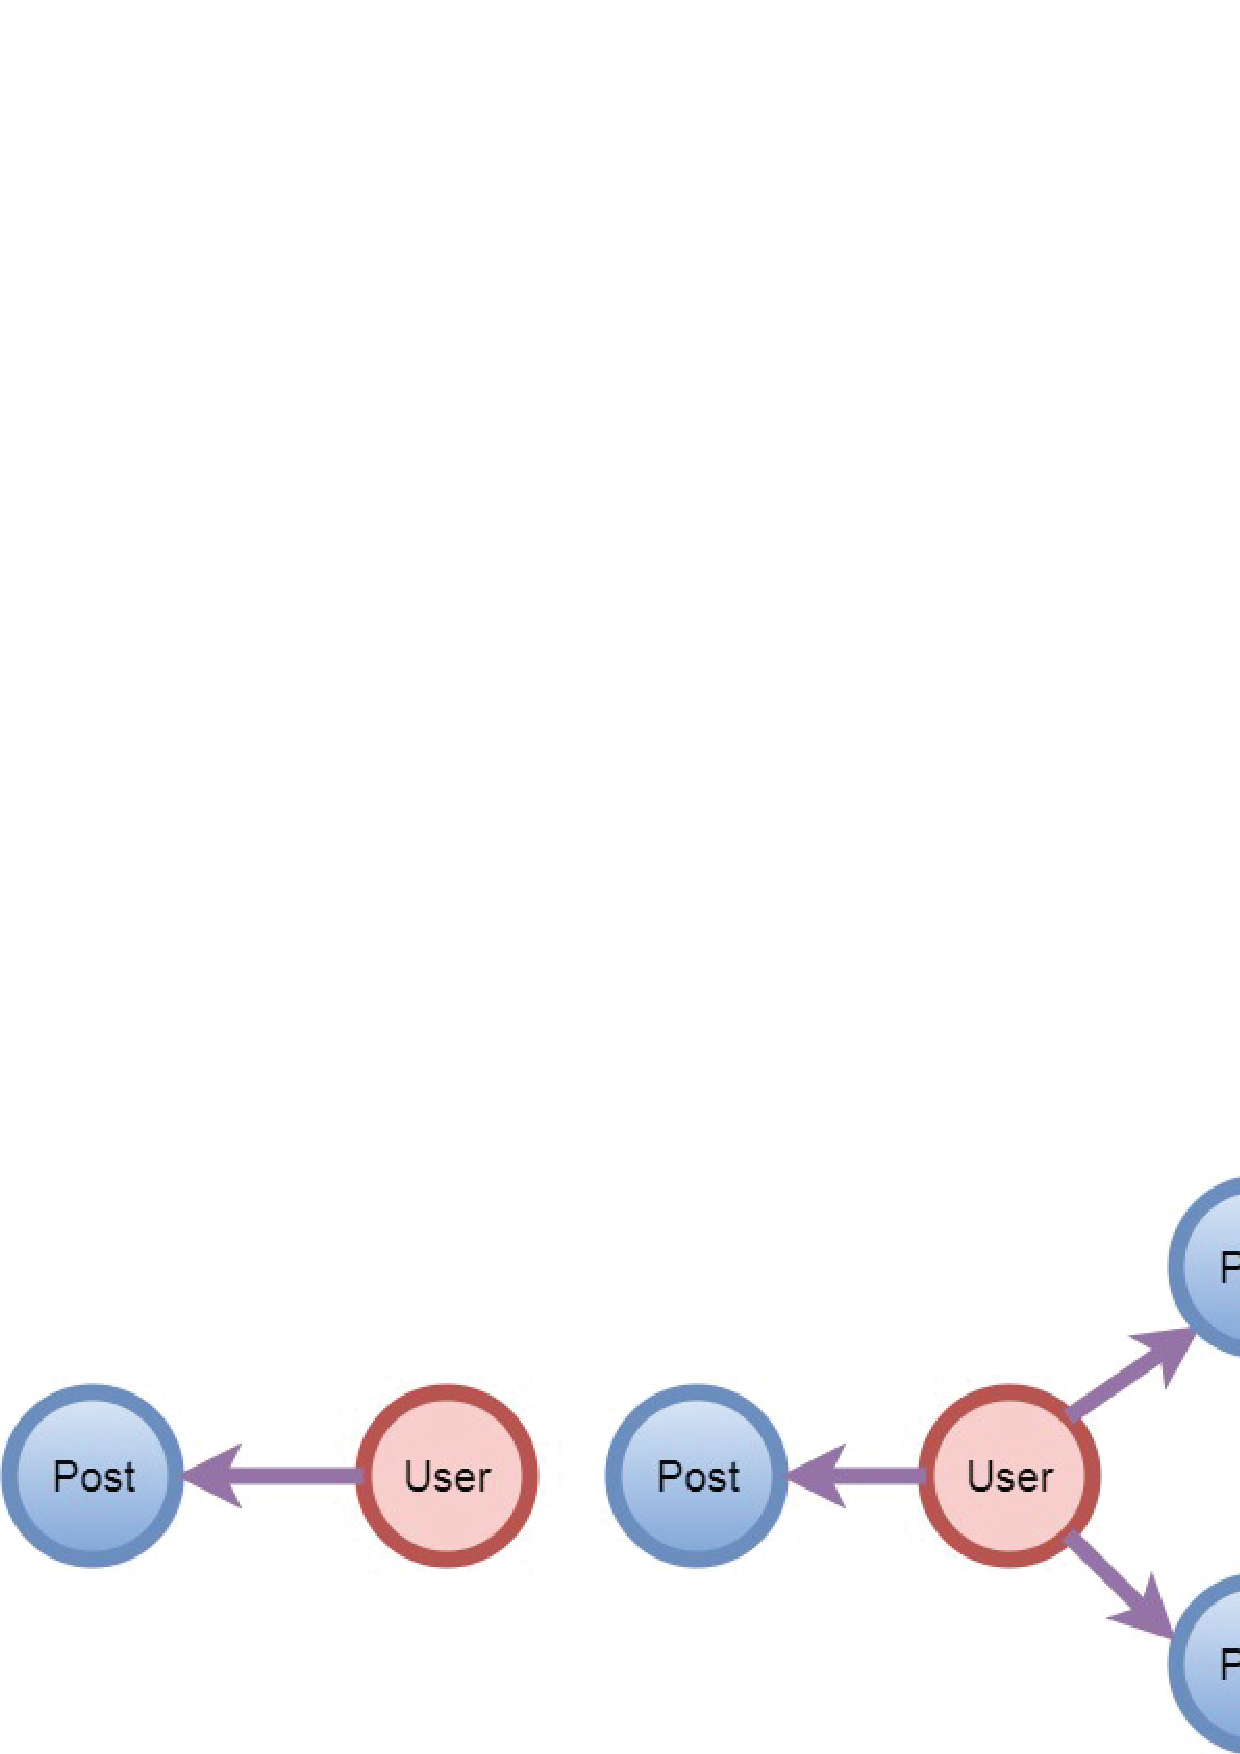
\includegraphics[scale=0.4]{pic/11.jpg}
\caption{A simple property graph modeling ``users post posts''(data graph).}
\label{fig:1}
\end{figure*}


%Besides nodes and edges, in property graph nodes and edges can have any number and type of properties. 


%For instance, in the exampling property graph,   That is, any node or edge could be freely attributed with any type of property. This makes a property graph very flexible in terms of property attribution.
 
%Property graph is an informative model as it contains not only nodes and edges, but properties of each individual node and edge as well. 

Note that although the property graph model does not enforce any restriction on what properties a node or edge can have, a highlevel abstraction describing the property relations, named the meta graph, is ofen defined in practice. Meta graph demonstrates the information of entities and entity correlations on a schema level, while data graph refers to the actual graph populated from the meta graph. Figure \ref{fig:2} and Figure \ref{fig:3} are the meta graph and a snapshot of the StackExchange graph, respectively. As shown in Figure \ref{fig:2}, there are three types of entities: User (in red), Post (in blue), and Tag (in green). Each user has a property named ``View'', each post has a property named ``Score'', and a property ``Tagname'' associated with each tag. There are two types of edges being  defined: User\_owns\_Post and Post\_hasTag\_Tag. 


\begin{figure*}[H]
\centering
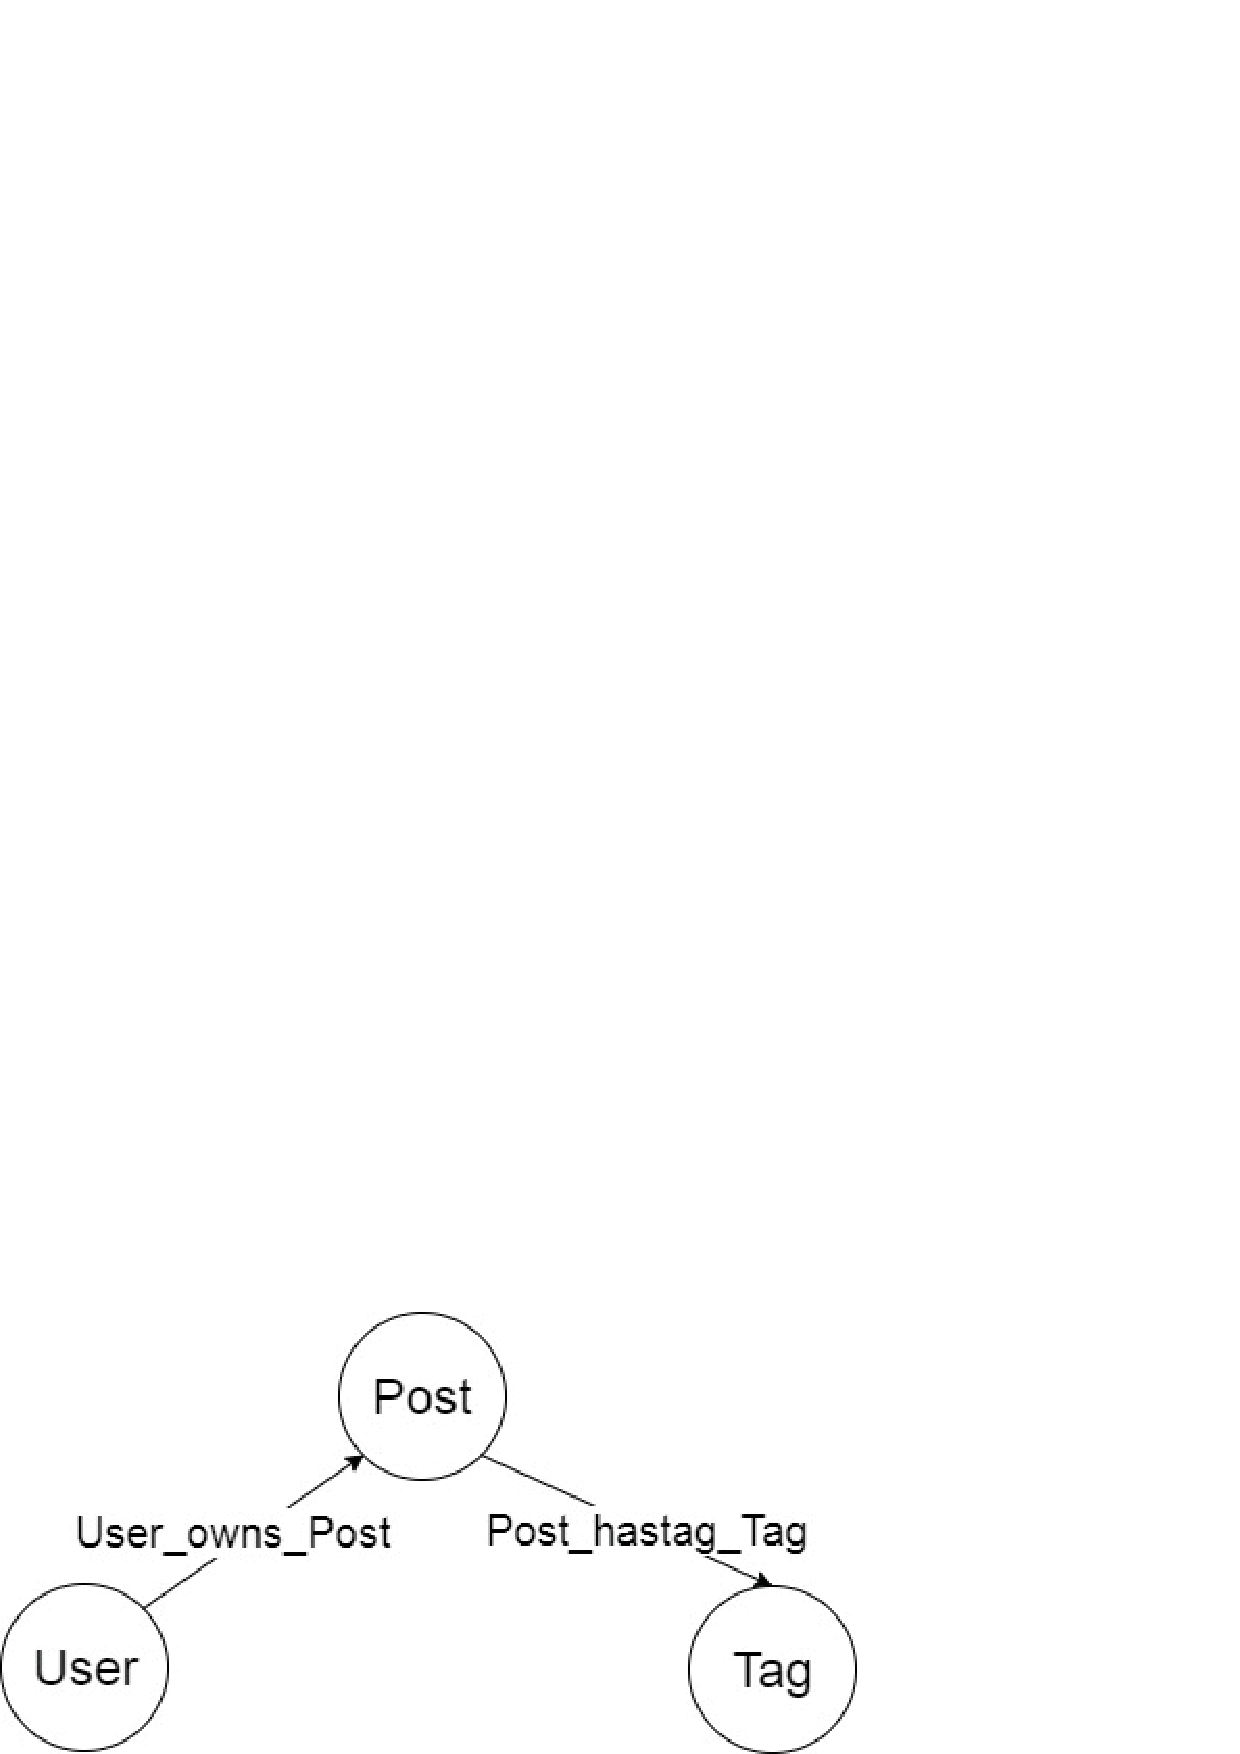
\includegraphics[scale=0.5]{pic/12.jpg}
\caption{Meta graph containing User, Post and Tag.}
\end{figure*}
 
\begin{figure*}[H]
\centering
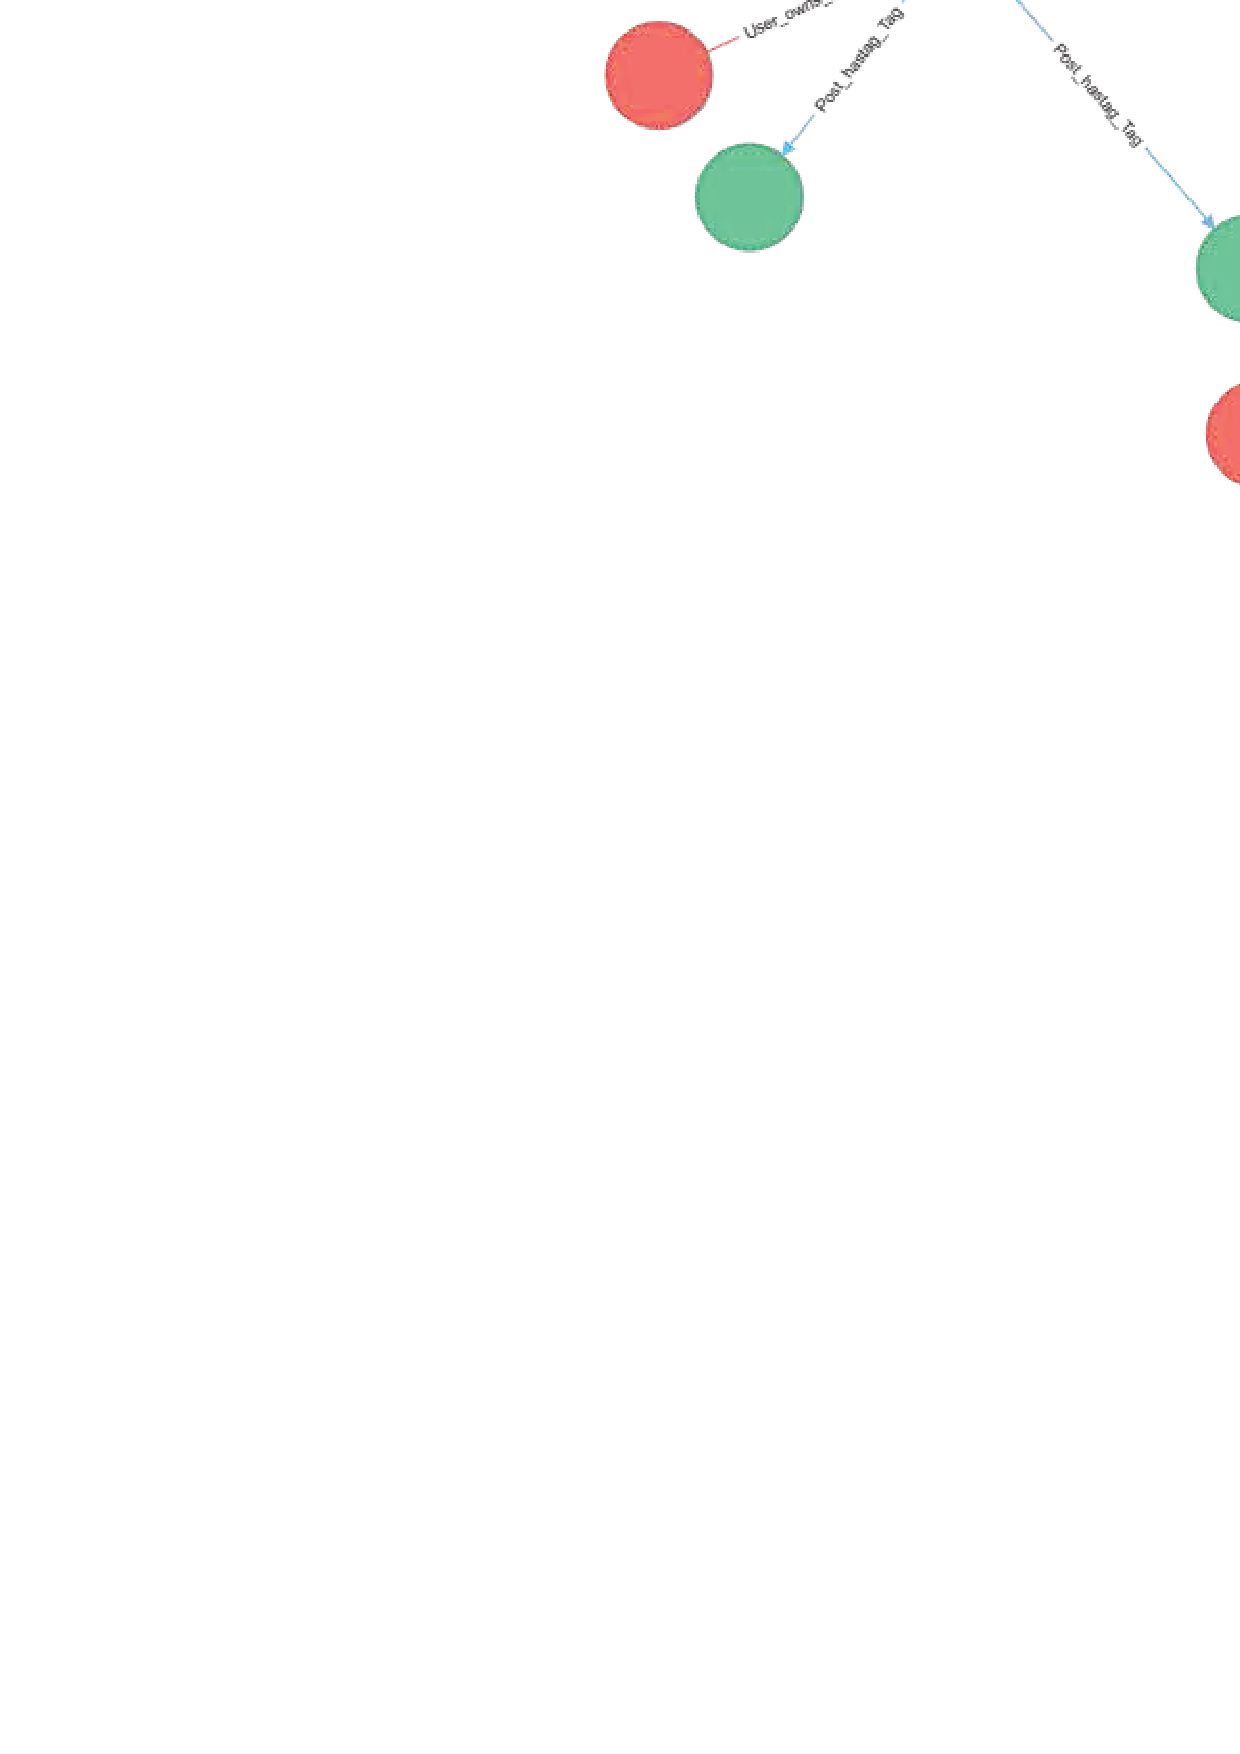
\includegraphics[scale=0.1]{pic/3.png}
\caption{A snapshot of data graph containing User, Post and Tag.}
\end{figure*}

%----------------------------------------------------------------------
\section{OLAP over Property Graph}
%----------------------------------------------------------------------
Among various kinds of queries, OLAP (Online analytical processing) queries play an important role in data analysis. 
\intodo{Add a few sentences to describe OLAP queries of the traditional database and warehousing applications. Showing it is important and we say performing OLAP on property graph is desired. }

In tradition databases and ware-housing, OLAP queries enable users to interactively perform aggregations on underlying data from different perspectives(combinations  of dimensions). There are three typical operations in OLAP. Roll-up operation allows user to view data in more details while drill-down operation does the opposite way. Slicing enables filtering on data. For instance, we can perform OLAP to analyze earning performance of an international company by different branch. We can perform drill-down operation by adding season as a dimension besides branch to take a closer look at profit performance of different branches in different seasons. In this case, OLAP serves as a tool for managers to better understand earning performance. 

Supporting efficient OLAP processing on property graphs grants users the power to perform insightful analysis over structured graph data. For example, on the StackExchange graph, users can study the correlation between the number of UpVotes and a post's score by using the following query:

\fbox{\emph{Get the average post score grouped by user’s upvotes.} }

 If the result shows a tight correlation, it suggests that an author’s upvotes can be used to estimate the quality of his or her post when a post is freshly posted and score of the post has not been settled.


Consider another example, using a property graph dataset on music industry,  one can issue the following query to evaluate a company's strategy to increase the share of young people's market.

\fbox{
\begin{minipage}{35em}
\emph{Get the total sum of music purchases by buyers at age 18-25 grouped by music company and month}
\end{minipage}
}


For simplicity, we call such kind of OLAP query workloads over property graphs as ``Graph OLAP''. As a matter of fact, graph OLAP has already been applied in various senerios like business analysis and decision making and it is attracting increasing research interests in the database community.



%----------------------------------------------------------------------
\section{Challenges of Graph OLAP}
%----------------------------------------------------------------------

%We know that Graph OLAP is important. However there are many challenges on this topic. One of the most challenging part is efficiency issue. 
\intodo{Here you should start with a paragraph saying "Supporing efficient OLAP is traditional RDBMS or warehousing applications is a well studied topic. There are abundent literature attacking this problem from virous different perspectives, e.g. data partition~\cite{}, view selection~\cite{}, partial materialization~\cite{}, .... However, there is very few research effort on the Graph OLAP. Existing literatures concerning OLAP workload over graph data either target on accelerating graph OLAP over a special subset of property graphs~\cite{}, or focus on generic highlevel topics, such as ... \cite{},  other than time efficiency issue of query processing."}

Supporting efficient OLAP in traditional RDBMS or warehousing applications is a well studied topic. There are abundent literature attacking this problem from virous different perspectives, e.g. data partition~\cite{DBLP:conf/ismis/CuzzocreaL12,}, view selection~\cite{DBLP:books/igi/Taniar10/LawrenceR10,}, partial materialization~\cite{DBLP:journals/kais/DrzadzewskiT16,}, .... However, there is very few research effort on the Graph OLAP. Existing literatures concerning OLAP workload over graph data either target on accelerating graph OLAP over a special subset of property graphs~\cite{DBLP:conf/sigmod/ZhaoLXH11}, or focus on generic highlevel topics, such as \cite{DBLP:conf/esws/MaaliCD15} \cite{DBLP:conf/icdm/ChenYZHY08},  other than time efficiency issue of query processing.

%From an academic point of view, most of OLAP studies reside in traditional relational data models, whereas studies on efficient graph OLAP are not enough. What's worse, current graph OLAP researches either  

Our empirical studis show that existing graph databases do not provide efficent support for graph OLAP, especially when the graph size scales to real-word practices, which usually contains over millions of nodes and edges. %Graph databases are databases that specialize in storage and processing of property graphs. However current graph databases are not satisfactory in terms of OLAP processing efficiency over large property graphs(often with more than millions of nodes and edges). 
To elaborate, Neo4j, a state-of-art graph database, processes OLAP queries in a rather straightforward manner: computing everything from scratch for each query without being aware of any history workloads. In an extreme case, even if we executed the same query repeatly with only minor change on value constraints, e.g., change the constraint of user's age from 20 to 22, the execution plan always stays the same and yields no execution time improvement.  

\begin{figure*}[H]
\centering
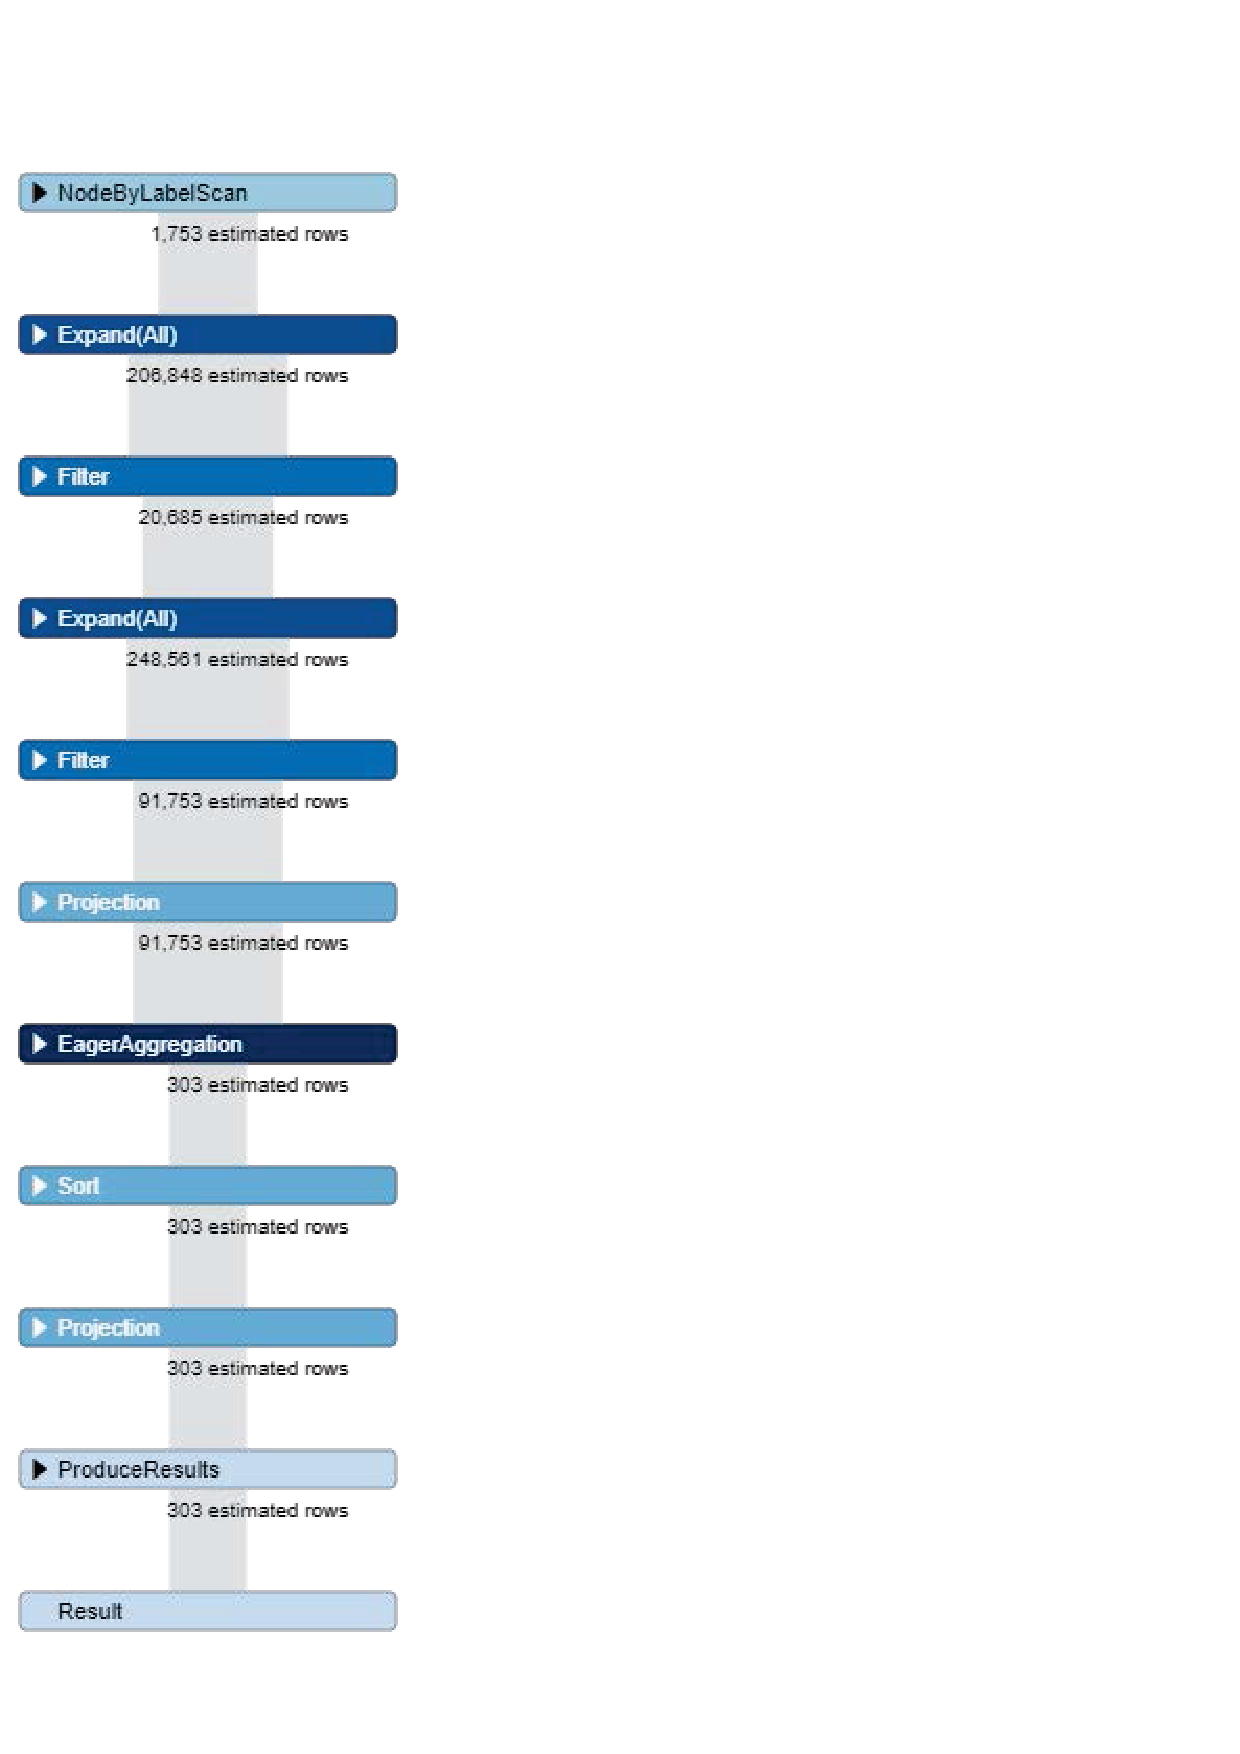
\includegraphics[scale=0.4]{pic/5.png}
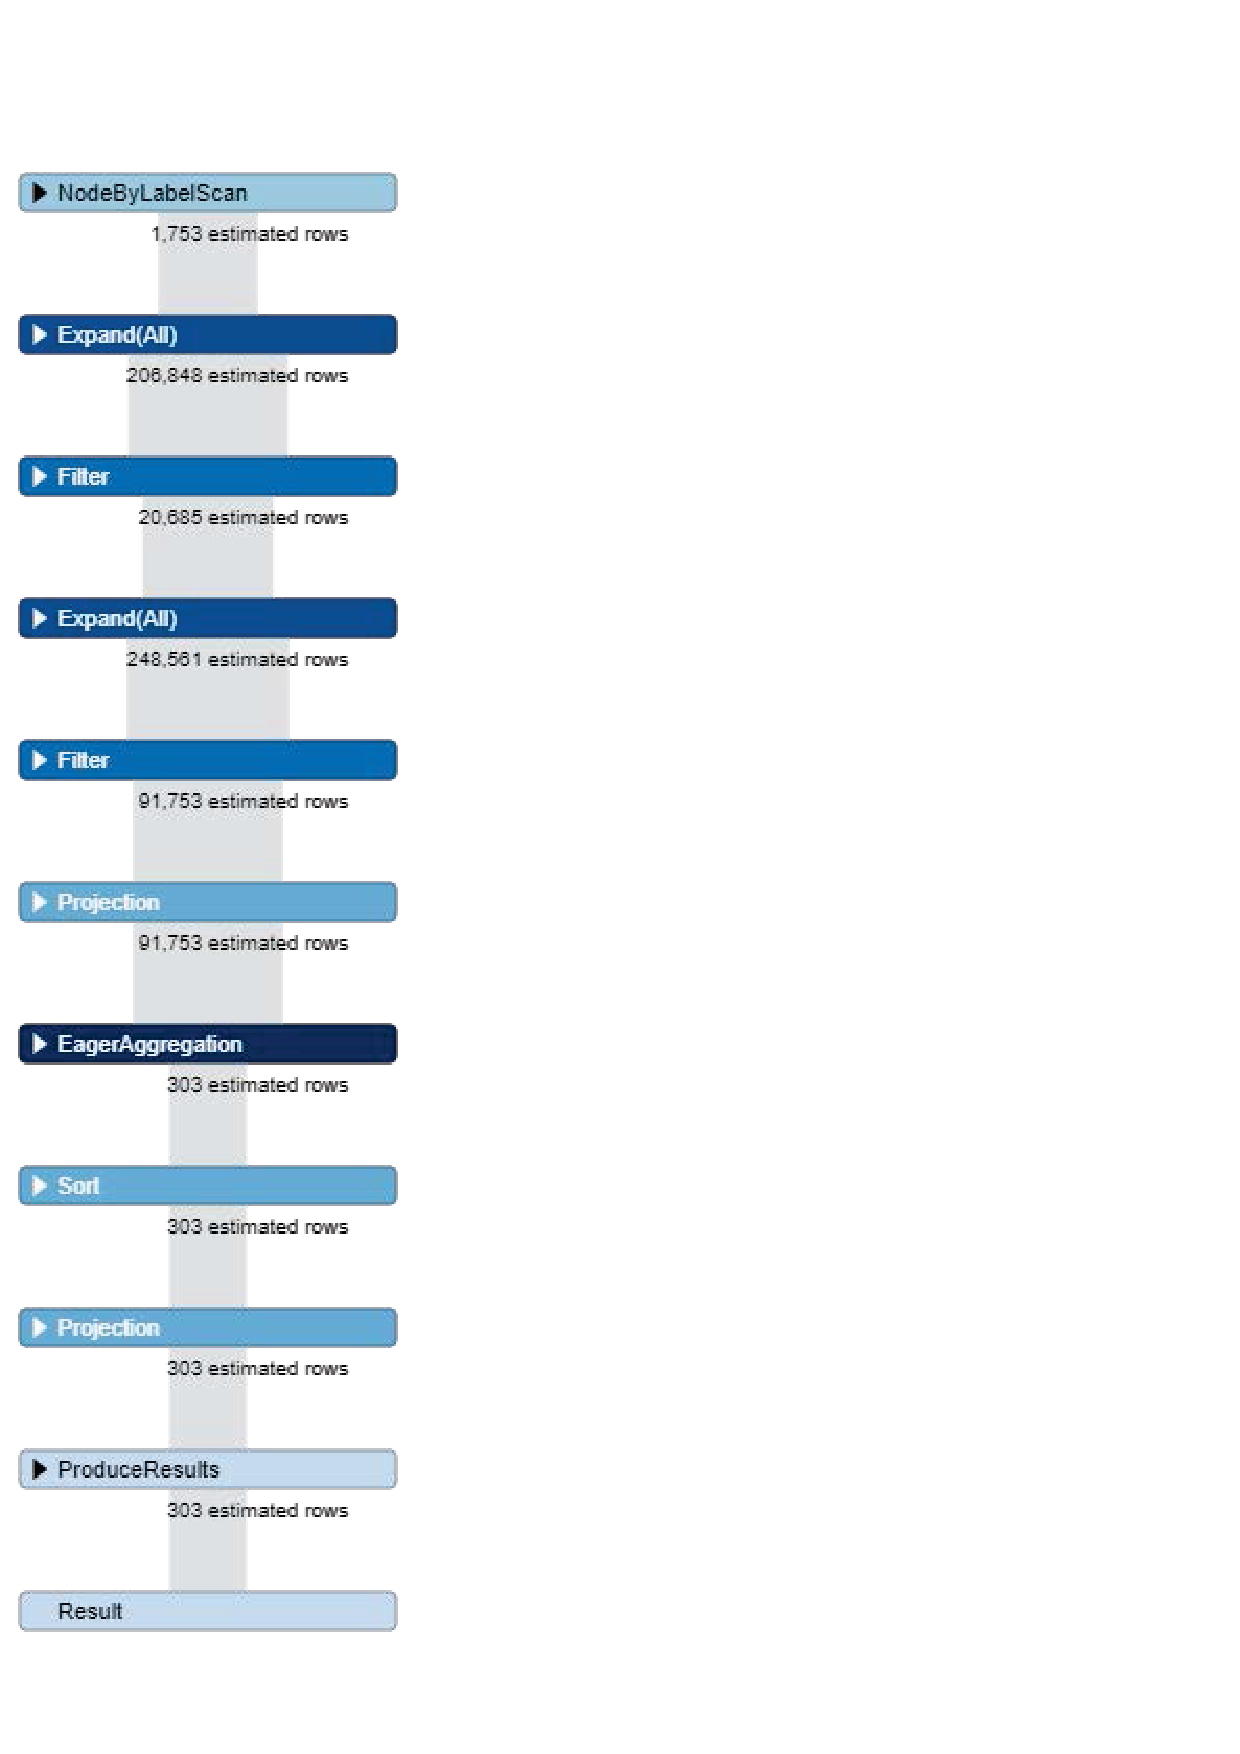
\includegraphics[scale=0.4]{pic/5.png}
\caption{Execution plans of Query \#3 for first time and fifth time.}

\end{figure*}

%This naive feature of always executing queries regardless of previous queries misses valuable information contained in previous workloads.
Valuable information extracted from history workload can be helpful to accelerate in-coming query processing. For example, the above exampling OLAP query on StackExchange graph dataset (of roughly 45GB in size) takes Neo4j more than 2 hours to process. It is frustrating for users to wait that long for the result of one single OLAP query, as it undermines interactivity which is one of the most distinctive features of OLAP. %Therefore we want to accelerate OLAP processing over large property graphs
\intodo{Now you should explain what you can learn from previous workloads, and how these knowledge can help you with future workloads.}

As a matter of fact, history workloads provide useful information for future workloads. This is because in real case users do not generate OLAP queries randomly. Instead users often tend to be interested in some specific ``hot'' structures on a meta graph level and some ``hot'' properties. Such interest is contained in history workload and can serve as an insightful hint on future workloads. Suppose we sacrifice some memory space and materialize ``hot'' structures and properties even before future queries arrive, future queries can be faster processed.  

\intodo{Then, you need a paragraph that describe the actual challenge. Because so far you only mentioned that using something from history workload is helpful, then the problem is how to extract these information, how to decide which information should be materialized espeically when there is a space constraint.}

We know that materialization on user's interested structures and properties results in benefit on future workload processing efficiency , and cost on memory space. The real challenge is how to design a score function to evaluate the trade-off  between such benefit and cost so that we can use the score function to select best materialization. Here best materialization refers to the case where we achieve best future workload acceleration with a given memory constraint for materialization.

%\begin{center}
%	\begin{tabular}{ | l | l | } 
%		\hline 
%		Query 	& Time	\\ \hline 
%		Query \#1	& \\ \hline
%		Query \#2	& \\ \hline
%		Query \#3	& \\ \hline
%	\end{tabular}
%	\end {center}
	
	


%----------------------------------------------------------------------
\section{Our Solution and Contributions}
%----------------------------------------------------------------------
To address the challenges discussed above, we propose a end-to-end solution for graph database to  support efficient  OLAP over large property graphs.

The essence of our solution is to precompute and materialize popular intermediate results that can be reused by future workloads. Intuitively, in real practice, most OLAP queries from the same client   tend to reside in several particular structures and properties (usually closely related with the topics that the client is interested in). Within a specific period of time, there are ``hot'' structures that the client tends to repeatedly investigate from different dimensions. Therefore, previous queries can be used as a good reference to discover structures and properties in which the client is particularly interested. 

%For instance, suppose a client just executed the exampling four queries, here is what we can learn from these four previous workload:

%Structure-wise: (User)-[creates]-$>$(Post) is frequently queried. We can tell that client is interested in how users create posts. Thus it is reasonable to guess that the user is likely to issue OLAP queries involving (User)-[creates]-$>$(Post) in following queries.
 
%Property-wise: User.UpVotes, Post.Score, User.Age, Tag.TagName etc. More specifically, \{User.UpVotes, Post.Score\} and \{User.Age, Tag.TagName\} are frequent combinations. Thus it makes sense to guess that these property combinations are likely to appear together in future queries.
 
%Intuitively, if we smartly select frequently queried structures and properties based on previous workload and materialize them, they might be covered in future queries and thus be used to accelerate processing. 
 
A good analogy of this is establishment of materialized views in relational databases and processing queries directly on materialized views. In relational databases, we are allowed to build materialized views on structures and attributes that we are interested in. Hopefully when future queries come, we can faster process them using pre-materialized views. Unfortunately, current graph databases do not support similar operations. 
 
%Therefore we propose a system that realizes automatic and smart pre-computing and materialization based on history workload, and utilize the materialized result to accelerate future query processing. 
 
There are two most important problems that we need to solve: 
 
One key issue is smart selection of ``materialized views''. We need to select and pre-compute those that are most beneficial for future queries. 
 
Another key issue is how to optimize a better execution plan for answering a future query efficiently using the precomputed materials.

\intodo{here you need to use a paragraph to explain how you select materialized views, e.g., you develop a cost function. Plus, you have a scheduling policy to execute subqueries in the most time efficient way. This part is particularly important, because reader need to briefly understand you overall solution from a high level perspective.}

For the first issue, we develop a score function to evaluate cost–performance ratio of a materialization. We propose a greedy  algorithm to  select candidate  based on their score(calculated from score function), one by one until memory limit is hit.

For the second issue, if a future query result can be directly produced using a materialization we simply do it. For other cases, we propose a scheduling policy to decompose a future query into substructures and join such substructures to produce final result.  

To highlight, we summurize our contributions in this thesis as follows:
\begin{itemize}
\item {We designed an end-to-end system that realizes structure-aware OLAP query processing on graph databases using precomputation based on previous workloads.}

\item We implemented our system on Neo4j.

\item We proposed our algorithm for smart selection of structures and cuboids to be precomputed.
 
\item We suggested different ways for future query processing. We tested their performances and gave explanations on the performance differences.
 
 \end{itemize}

The following contents are organized as follows:
 we discuss the preliminaries and related work in Chapter 2. Followed by the background knowledge about  OLAP, graph databases, and Neo4j, we give a summarization of existing literatures concerning OLAP queries over graph data. In Chapter 3 we explain our solution framework and system design in details. We present the experiment design and result disucssion in Chapter 4. Chapter 5 concludes this thesis with highlight on opening questions and future work.




%======================================================================
\chapter{Background and Related Work}
%======================================================================
%----------------------------------------------------------------------
\section{More on Property Graph Model}
%----------------------------------------------------------------------
We have introduced about property graph model in Introduction part. We know that in property graph model, each node and edge could have arbitary number and type of properties. A type of property is represented by 

NodeType.PropertyType

For instance User.Age represents "Age" property on "User" node.

In order to identify a node or edge, a unique ID is assigned to each node and edge.  In this thesis we represent a type of property by 

ID(node) or ID(edge)

to represent unique ID of a node or edge.

%----------------------------------------------------------------------
\section{Graph OLAP}
%----------------------------------------------------------------------
Three key elements of a graph OLAP are structure, dimension, and measure. Taking Query \#1 as an example: 
 
Question: 	Does high upvotes of a user indicates a high-quality post? 
Query: 		Get average post score grouped by user’s upvotes. 
 
This query is on all the following structures:

\begin {figure}[H]
\centering
\includegraphics[scale=1]{pic/21.png}
\end{figure}

We say that (User)-[User\_owns\_post]->(Post) is the structure of Query \#1.
The query is aggregated by (grouped by) user’s upvotes. We say that {User.Upvotes} is the dimension of Query \#1.
The query is aggregated on avarage of post’s score.  We say that {AVG(Post.Score)} is the meansure of Query \#1. 
 
Similarly, for Query \#2:

Question: 	Similar to Query \#1. But this time we want to take a closer look at Query \#1 for different types of questions. 

Query: 		Get average post score grouped by user’s upvotes and post’s post types. 

Structure:	(User)-[User\_ownspost]-(Post)

Dimensions:	{User.Upvotes, Post.PostTypeId}

Measures:	{AVG(Post.Score)}
 
Notice that Query \#2 adds Post.PostTypeId to Query \#1’s dimensions. That is to say, Query \#2 asks for a more detailed partitions over dimentions. We call Query \#2 a drill-down from Query \#1, and  Query \#1 a roll-up from Query \#2. Such roll-up and drill-down operations allow us to navigate up and down through the dimensional lattice of all possible property combinations. 

\begin {figure}[H]
\centering
\includegraphics[scale=1]{pic/22.png}
\end{figure}

Query \#3:

Question: 	In year 2017, which is the weighted average age of users? For instance is ‘python’ more trendy than ‘c’ among young users?
 
Query: 		Get average user age grouped by users’ 2017 posts’ tags. 

Structure:	(User)-[User\_owns\_post]-(Post)-[Post\_hastag\_Tag]-(Tag)

Dimensions:	{Tag.Tagname}

Measures:	{AVG(User.Age)}
 
In Query \#3, a requirement that post must be created in year 2017 picks out a particular subset of  all (User)-[User\_owns\_post]-(Post)-[Post\_hastag\_Tag]-(Tag) candidates. In OLAP this is called “slicing” operation. Slicing operation allows users to view the data with filtering requirements on selected properties. 
 
In this thesis we call {Post.Year=2017} a "slicing condition" of Query \#3.
 
To summarize, graph OLAP allows clients to aggregate different structures, over different dimensions, on different measures. Clients can change their views by performing roll-up, drill-down, and slicing freely and interactively.


%----------------------------------------------------------------------
\section{Graph Databases}
%----------------------------------------------------------------------


We have discussed about property graphs and OLAP over property graphs on a high level. This leads us to a question. How are property graphs actually stored and managed in database systems? 
 
There are two major types of databases that store and process graph data: traditional relational databases and graph databases. 
 
Relational databases adopt traditional ways of modeling data in form of entity and relationship tables. For instance, for the following property graph, which consists 1 user and his or her 3 posts. A relational database stores the property graph as 3 tables:

\begin {figure}[H]
\centering
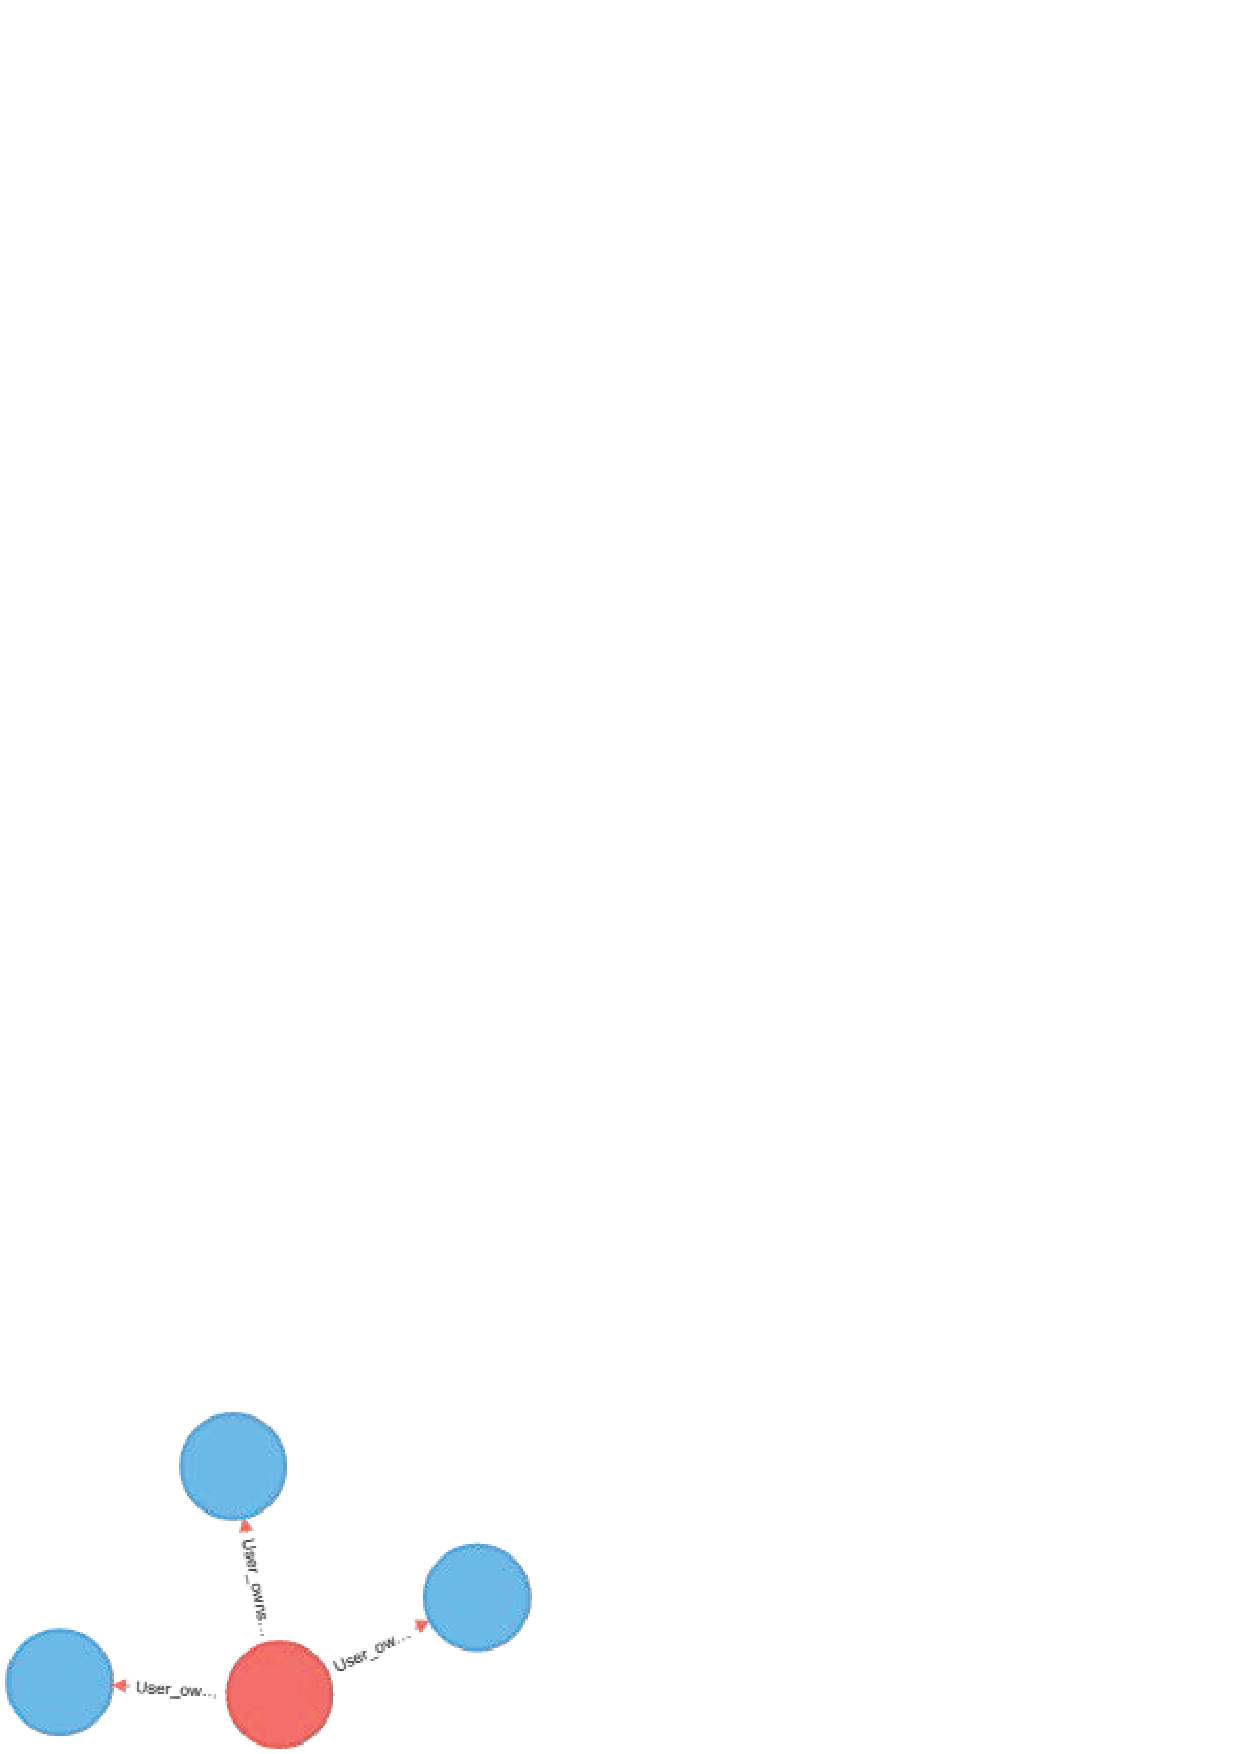
\includegraphics[scale=0.9]{pic/4.png}
\end{figure}

Table-User
\begin{center}
\begin{tabular}{ l | l }  
	Uid	&{All user properties}	\\ \hline 
	1	&{Property values} \\
\end{tabular}
\end {center}

Table-Post
\begin{center}
	\begin{tabular}{ l | l }  
		Pid	& {All post properties}	\\ \hline 
		1	&{Property values} \\
		2	&{Property values} \\
		3	&{Property values} \\
	\end{tabular}
	\end {center}	
 
Table-Owns
\begin{center}
	\begin{tabular}{ l | l }  
		Uid	& Pid	\\ \hline 
		1	&1 \\
		1	&2 \\
		1	&3 \\
	\end{tabular}
	\end {center}

 
There are two drawbacks of storing property graphs in relational databases. First, each node or edge of in property graph could have arbitrary types of properties. However, schemas of relational tables restrict nodes or edges of a same type to have a uniform set of properties (attributes). Second and more importantly, edges are not stored as a separate table. For instance, we cannot directly query all the posts of a given user without joining User and Own tables in the above example.
 
Graph databases solve the above two issues by directly adopting property graph structures to store data. In graph databases, edges are stored not as independant tables but directly attached to related nodes using data structures such as adjacency lists. Many graph database applications have been implemented and commercialized. One of the popular ones is Neo4j.
 
Relational databases and graph databases both have their own strengths in term of query processing. However it is generally accepted that graph databases perform better at property graph data processing as it conforms more with the actual graph structure. 

%----------------------------------------------------------------------
\section{Neo4j}
%----------------------------------------------------------------------
Neo4j is one of the most popular graph databases which holds atomicity, consistency, isolation, durability (ACID). 
 
Instances are modeled and stored as  property graphs in Neo4j. Like other graph databases, edges are not stored as physically separate tables, but directly attached to their nodes. One special thing about Noe4j’s property graph is that its nodes and edges can be labeled with any number of labels (similar to entity and relationship types). For instance a node referring to a student could have various labels such as “student”, “people” etc. 

Cypher is Neo4j’s query language, which is expressive and simple. Here are some examples of Cypher queries:

Aggregation query: For answers(Post.PostTypeId=2), what is the average score group by different user upvotes?
 
match (u:User)-[r:User\_owns\_Post]->(p:Post) where p.PostTypeId="2" return u.Upvotes, AVG(p.Score)
 
Here “User” and “Post” are labels, PostTypeId and Score are properties of “Post” node, “Upvotes” is property of “User” node.
 
Neo4j is written in Java. While applications in various languages could interact the server by issuing queries with its own BOLT protocol(which is binary and more efficient than HTTP).  

\begin {figure}[H]
\centering
\includegraphics[scale=0.4]{pic/23.png}
\end{figure}


%----------------------------------------------------------------------
\section{Graph Aggregation Paper Summary}
%----------------------------------------------------------------------

Numerous papers have been published on graph aggregation. 

Cube-based [1] proposes the concept of  graphs enriched by cubes. Each node and edge of the considered network are described by a cube. It allows the user to quickly analyze the information summa-
rized into cubes. It works well in slowly changing dimension problem in OLAP analysis.

Gagg [2] introduces an RDF graph aggregation operator that is both expressive and flexible. It provides a formal definition of Gagg on top of SPARQL Algebra and defines its operational semantics and describe an algorithm to answer graph aggregation queries. Gagg achieves significant improvements in performance compared to plain-SPARQL graph aggregation.

Pagrol [3] provides an efficient MapReduce-based parallel graph
cubing algorithm, MRGraph-Cubing, to compute the graph cube
for an attributed graph. 

Graph Cube [4] introduces Graph Cube, a new data warehousing model that supports OLAP queries effectively on large multidimensional networks. It takes account of both attribute aggregation and structure summarization of the networks. In order to deal with “curse of dimensions”, a greedy algorithm framework is introduced for partial materialization of cuboids.

Snapshot [5] studies dimensions and measures in the graph OLAP scenario and furthermore develops a conceptual framework for data cubes on graphs. It differentiates different types of measures(distributive and holistic etc) by their properties during aggregation. It looks into different semantics of OLAP operations, and classifies the framework into two major subcases: informational OLAP and topological OLAP. It points out a graph cube can be fully or partially materialized by calculating a special kind of measure called aggregated graph. 


We summarize some of the most related ones as follows:
 
 \begin{center}
 	\begin{tabular}{ | c | c | c | c | c |  } 
 		\hline 
 		 & Input graph & Query pattern & Layer structure & Highlight\\ \hline Cube-based [1] & property graph & simple relation & yes & cubes on edges and nodes\\ \hline Gagg [2] & property graph & all exact-match patterns & no & structural patterns\\ \hline Pagrol [3] & property graph & edge and node attributes & yes & Map-Reduce distributed computing\\ \hline Graph Cube [4] & homogenous nodes and edges & node attributes & yes & partial materialization algorithm\\ \hline Snapshot [5] & property graph & edge and node attributes & yes & distributive and holistic measures\\ \hline 
 	\end{tabular}
 	\end {center}

 
 
From the summary we can categorize the papers into two kinds: 
 
First, like Graph Cube[4], focuses on a simple subset of property graphs(e.g. graphs with only homogenous nodes and edges) and propose optimizations on OLAP query processing. The optimizations are attribute-aware, and since the nodes and edges are of only one kind queries over different structures and structure-aware optimizations are out of the scope. 
 
Second, like Gagg [2], focus on an abstract high-level framework that process generic queries over generic property graphs. However, query optimizations are not focused.  
 
Therefore it is very meaningful to explore faster structure-aware OLAP processing over general property graphs.



%----------------------------------------------------------------------
\section{Graph Cube}
%----------------------------------------------------------------------

In Graph Cube [4], concepts of graph cube is introduced. Given a particular structure S, a property set P, and measure set M. We can aggregate over S on 2\^{}|P| different combinations of dimensions. These 2\^{}|P| queries can be mapped as a lattice structure, where each combination of dimensions corresponds to a cuboid in the lattice. We call the lattice structure of these 2\^{}|P| queries a graph cube.

\begin {figure}[H]
\centering
\includegraphics[scale=1]{pic/22.png}
\end{figure}

It has been pointed out that as long as if domain of measure is within \{count, sum, average\} and M contains count(*), the following feature holds:
 
Given any two cuboids C1 and C2 from the same graph cube, as long as dimension(C2) is a subset of dimension(C1), result of C1 can be used to generate result of C2. This is to say once a cuboid is materialized, all roll-up operations from this cuboid could be processed simply by scanning the materialized cuboid result. This will dramatically decrease roll-up operation time compared to aggregation from data graph(often of larger size, disk I/O), scanning materialized cuboid result(often of smaller size) is often much faster.


 
Ideally we can materialize all cuboids. But when number of dimension is large, number of cuboids grows exponentially, making total materialization impossible due to overwhelming space cost. To solve this Graph Cube [4] proposed a partial materialization algorithm on graph cube. It is a greedy algorithm and the score function is based on benefits of deduction of total computation cost.



%======================================================================
\chapter{Problem Definition}
%======================================================================
In this section, we first illustrate the terminology and notations adopted in this work. Then we formally define the problem of efficient OLAP query processing. 

%----------------------------------------------------------------------
\section{Terminologies}
%----------------------------------------------------------------------

This section gives definations and notations of property graph, queries, materializations. Besides, we introduce concepts of ``cuboid'' and ``subsubstrcutre'', which are two types of materializaitons we will use in our solution. 

\subsection{Defination of Property Graph}
We define a property graph as $G(V, Vid, E, Eid, A, L, f)$ where
\begin{itemize} 
\item $V$ is a set of nodes. $Vid$ is set of unique IDs of $V$.
\item $E$ is a set of edges. $E \subseteq V * V$. $Eid$ is set of unique IDs of $E$.
\item $A$ is a set of properties.
\item $L$ is a set of labels.
\item $f$ is mapping function that maps $V$ and $E$ to $A$, $L$, $Vid$ and $Eid$. 

$f_{VA}: \{V_{i} \rightarrow A_{i}\}, V_{i}\in V, A_{i} \subseteq A$ , maps each node to its properties.

$f_{VL}: \{V_{i} \rightarrow L_{i}\}, V_{i}\in V, L_{i} \subseteq L$ , maps each node to its labels.

$f_{EA}: \{E_{i} \rightarrow A_{i}\}, E_{i}\in E, L_{i} \subseteq A$ , maps each edge to its properties.

$f_{EA}: \{E_{i} \rightarrow L_{i}\}, E_{i}\in E, L_{i} \subseteq L$ , maps each edge to its labels.

$f_{VID}: \{V_{i} \rightarrow Vid_{i}\}, V_{i}\in V, Vid_{i} \subseteq N$ , maps each node to its unique ID.

$f_{EID}: \{E_{i} \rightarrow Eid_{i}\}, V_{i}\in V, Eid_{i} \subseteq N$ , maps each edge to its unique ID.

\end{itemize} 

\subsection{Notations on OLAP Query}

As discussed before, Four elements of a graph OLAP query are \textit{Structure}, \textit{Dimension}, \textit{Measure}, and \textit{Slicing Condition}(optional). We will introduce how we represent these four elements and an OLAP query. We will use Query \#3 in Chapter 2 as an example.

\textbf{\textit{Structure:}} A \textit{strucuture} consists of \textit{edges}. We write a \textit{structure} by listing all its \textit{edges} seperated by comma, where an \textit{edge} is represented by 

\fbox{
	\textit{Starting Node Label- Edge Label- Ending Node Label} 
}

For instance, Query \#3's \textit{structure} as shown in \ref{fig:2:3} is written as 

\textit{``User-owns-Post, Post-has-Tag''}



\textbf{\textit{Dimension:}} A
\textit{Dimension} is written by listing all properties that act as dimensions in an OLAP query.

Query \#3's \textit{dimension} is written as

\textit{``Tag.Tagname''}

\textbf{\textit{Measure:}} We focus on three most common types of \textit{measure}: \textit{COUNT(*), SUM and AVG. }

Query \#3's \textit{measure} is written as

\textit{``AVG(User.Age)''}


\textbf{\textit{Slicing Conditions:}} A \textit{Slicing Conditions} is written as 

\fbox{
$Property = value$
}

Query \#3's \textit{slicing conditions} is written as

\textit{``Post.Year=2017''}

\textbf{\textit{OLAP query:}} With the four elements ready, we write an entire OLAP query as 

\fbox{
	\textbf{\textit{Structure : Dimension, Measure, Slicing Condition}}
}

Query \#3 is written as 

fbox{
\textit{User-owns-Post, Post-has-Tag: Tag.Tagname, AVG(User.Age), Post.Year=2017
}

where \textit{User-owns-Post, Post-has-Tag} referring to  \textit{structure}, \textit{Tag.Tagname} referring to \textit{dimension},\textit{ AVG(User.Age) } referring to \textit{measure}, {Post.Year=2017} referring to \textit{slicing condition}. Note that since \textit{dimension}, \textit{measure} and \textit{slicing condition} are written in different forms, it is easy to distinguish them even if they are all listed together.


 \textbf{\textit{Features of a query:}} For a query q, we use ``q.properties'' to refer to a set of \textbf{all properties} in \textit{Dimension, Measure, and Slicing Condition} of q. We use ``q.structure'' to refer to structure of q.

 \textit{Query \#3.properties=\{Tag.Tagname, User.Age, Post.Year\}}
 
 \textit{q.structure= User-owns-Post, Post-has-Tag}



\subsection{Materialization: Cuboid vs Substructures}

We want to accerlerate OLAP by materializations from previous workload. We use

\fbox{
	\textbf{\textit{\$Query}} 
}

to refer to materializaiton of a $Query$.

As we mentioned before, in a property graph each node and edge has a unique ID, which can be treated as a special property. Whether a materialization keeps unique ID is an important issue, as keeping unique ID often increases space cost of a materialization. We categorize two types of materializaitons, ``cuboid'' and ``substructure'', based on whether unique IDs of nodes and(or) edges are kept or not. To better understand ``cuboid'' and ``substructure'', let's look at the following example.


Suppose we have following previous workload and future workload:

Previous workload \#1 User-owns-Post: User.Age\\
Previous workload \#2 User-owns-Post: User.Age, (AVG)Post.Score\\
Future workload \#1 User-owns-Post: (AVG)User.Age, Post.Score	\\
Future workload \#2 User-owns-Post, Post-has-Tag: User.Age, Tag.TagName




%User-owns-Post: User.Age
%
%User-owns-Post: User.Age, (AVG)Post.Score
%
%User-owns-Post, Post-has-Tag: User.Age, Tag.TagName

We can tell that the user is most interested in  \textit{User-owns-Post} structure. \{User.Age, Post.Score\} is the set of properties that are involved in queries over \textit{User-owns-Post} . We can build a cuboid lattice of all combinations of  \{User.Age, Post.Score\}. Materialization of base cuboid of the lattice is

\fbox{
\textit{\$User-owns-Post: User.Age, Post.Score, COUNT(*)}
}

\textit{\$User-owns-Post: User.Age, Post.Score, COUNT(*)} is useful for future workload \#1. We can process future workload \#1 by aggregation over \textit{\$User-owns-Post: User.Age, Post.Score, COUNT(*)}. We call such materilization a \textbf{``cuboid''}.


However, \textit{\$User-owns-Post: User.Age, Post.Score, COUNT(*)} is not useful for future workload \#2. The reason is that they have different \textit{structures}.


If we add ID(Post) into \textit{dimension} and materialize \textit{\$User-owns-Post: User.Age, Post.Score, ID(Post) COUNT(*)}, \textit{Post} is ``activated'' to be able to join with other materializations containing \textit{Post} and produce results for OLAP over more complicated \textit{structures}. For instance, future workload \#2 can be processed by 


1.joining \textit{\$User-owns-Post: User.Age, Post.Score, ID(Post) COUNT(*)} and \textit{\$Post-has-Tag: ID(Post), Tag.TagName, COUNT(*)} on ID(Post)

2.aggregation on \{User.Age, Tag.TagName\}. 

In this case, we only need to fetch \textit{\$Post-has-Tag: ID(Post), Tag.TagName, COUNT(*)} from database to produce result for future workload \#2. We call such materialization with ID(s) in \textit{dimension} \textbf{``substructure''}. 

Note that cuboids can only be used in queries with exactly the same structure. They can be be scanned for more aggregated dimension combinations(drill-down operations) but they are not useful for queries with different \textit{structures}. 

Substructures can be used to join with other materializations to help with future queries of various types of \textit{structures}.
The drawback is that structures are generally more space-costly than cuboids, as IDs are unique keys. The trade-off between cuboids and substructures is \textbf{\textit{space vs joining potential}}.

\ref{Table:3:1} gives a summary of comparisions between ``cuboid'' and ``substructure''. 

 \begin{table}
	\footnotesize
\begin {center}
\begin{tabular}{ | l | l | l |}
	\hline
 &Cuboid&Substructure\\ \hline
 Dimension& Only properties& Properties and ID(s)\\ \hline
 Space Cost& ``Low''&``High''\\ \hline
 Potential benefit& Aggregation& Aggregation \& Joining\\ \hline
\end{tabular}
\end {center}
\caption{Comparisons between Cuboid and Substructure.}
\label{Table:3:1}
\end{table}


%----------------------------------------------------------------------
\section{Problem Definition}
%----------------------------------------------------------------------

Our target is to faster process future OLAP workload using materializations computed based on previous workload. We can divide our goal in two steps. 
\begin{itemize}
	\item Materializaiton Step: clever selection of views for materialization. 
	\item Query Processing Step: processing future queries in shortest time(using materializaitons). 
\end{itemize} 

Materializaiton Step requires us to solve ``Materialization Selection Problem''. Query Processing Step requires us to solve ``Processing Plan Problem''. We give definations for these two problems as follows.

\textbf{``Materialization Selection Problem'':}

Using materialization is good for query efficiency, but comes with a storage cost. So we want to study the problem of how to best utilize materialization within a space budget limit $\sigma$. 


\\
We define ``Materialization Selection Problem'' as

Given a property graph dataset G, a set of previous queires P on G, space limit $\sigma$, find cuboids C and substructures S, $\displaystyle{\sum_{c_{i}\in C}c_{i}.space} + 
\displaystyle{\sum_{s_{i}\in S}s_{i}.space} 
\leq \sigma
$, so that $\displaystyle{\sum_{p_{i}\in P}estimatedProcessingTime(G, p_{i}, C, S)}$  is minimized.

Here $estimatedProcessingTime(p_{i}, C, S)}$ is a function for estimation of query processing time of $p_{i}$ on G using materializations of C and S.

%Is ``Processing Plan Problem'' even considered as a problem?
 
\textbf{``Processing Plan Problem'':}

We define ``Processing Plan Problem'' as


Given a property graph dataset G, a future query q, materialized cuboids C and substructures S, find a processing plan $process(G, q, C, S)$, so that $process(G, q, C, S).executionTime$ is minimized.



%======================================================================
\chapter{Solution}
%======================================================================
%!TEX root = main.tex

In this chapter, we present our complete solution towards efficient OLAP query processing over property graphs. For comprehensive presentation, we first illustrate the overall solution framework in Section \ref{s:4.1}. Then we present our strategy for materialized view selection, as well as the execution planning for query processing in Section \ref{Materialization Part} and \ref{Future Query Processing Part}, respectively.



%----------------------------------------------------------------------
\section{Solution Framework Overview}
\label{s:4.1}
%----------------------------------------------------------------------

\begin{figure}[H]
	\centering
	\includegraphics[scale=0.5]{pic/frame.pdf}
	\caption{Solution framework.}
	\label{Solution framework}
\end{figure}

Figure \ref{Solution framework} describes the overall solution framework. Two dashed line rectangles represents the major components of our solution: materialization and query processing. Materialization takes previous workload as input and materializes cuboids and substructures which are beneficial for future workload processing. We adopt a straightforward best effort approach for materialization. Intuitively, we first partition previous queries into ``hot'' queries and ``less hot'' queries based on the frequency count of their structures. Modules CubePlanner and StructurePlanner take ``hot'' queries and ``less hot'' queries as input and produce cuboids and substructures (in form of tables) for materialization respectively. More details are left to Section \ref{Overview of Materialization Part}, where we will explain the intuition of categorization of ``hot'' and ``less hot'' queries, as well as the reason of passing them to different planners.  Query processing component takes incoming queries as input and returns results. Briefly, the workflow of query processing is the following. If a new query happens to contain a ``hot'' structure, we consult cuboid materializations to see if it can be directly answered by aggregation over a cuboid materialization. In this case, cuboid materialization will be used. Otherwise, if the query cannot be directly answered by any materialized cuboid, we consider available materialized substructures by decomposing the query into substructures for join. Note that if required substructure is not materialized, on the fly data fetching from the graph database server is mandatory. %In this case, substructure materializations will be used.

%We will discuss ``Materialization Part'' in Section \ref{Materialization Part} and ``Future Query Processing Part'' in Section \ref{Future Query Processing Part}.




%----------------------------------------------------------------------
\section{Materialized View Selection}
\label{Materialization Part}
%----------------------------------------------------------------------

%We will discuss materialized view selection in this section. We will first give an overview of materialized view selection and then focus on cuboid and substructure selections respectively.
Materialized view selection is a research problem that has attracted significant attention in traditional RDBMS community. However, the fundamental difference between the relational model and the property graph model makes materialization of graph database an interesting topic to explore. This is mainly because \textit{structure} plays an important role in a query over a property graph. One materialized view may affect the benefits of other ones (e.g., when their \textit{structures} overlap). Therefore combinational benefit for a set of materialized views is not a simple sum of benefits for each one of them. As briefly illustrated before, we consider two types of materializations for efficient OLAP query processing: cuboids and substructures. In this section, we first elaborate the essential heuristic of selecting cuboids and substructures. Then we detail the approaches taken for different types of materializations.

%----------------------------------------------------------------------
\subsection{Overview of Materialized View Selection}
\label{Overview of Materialization Part}
%----------------------------------------------------------------------
In Section \ref{Materialization: Cuboid vs Substructures}, we discussed the trade-off between cuboids and substructures. We know that utilization of a cuboid materialization requires future queries to have exactly the same structure as the materialized cuboid. Therefore, it is only reasonable to materialize a cuboid %if TheIt is wise that we materialize a cuboid only
when we are confident that the same structure is likely to be ``hit'' by future queries. Otherwise, it is simply a waste of space to materialize cuboids that would be rarely ``hit''. On the contrary, substructures do not have such strict structural match requirement. A substructure can be used as long as it appears in a future query.

Considering the different features of cuboids and substructures, we take the following strategy for materialized view selection.
%We make our materialization policy based on such different features of cuboids and substructures.
We first perform a frequency count of previous queries. If more than $\omega$ queries shares the same structure, where $\omega$ is a predefined frequency threshold, this structure is considered to be a \emph{hot structure} and would be passed on to the \emph{CubePlanner} module for cuboid selection. Queries that do not have \emph{hot structures} are passed to \emph{StructurePlanner} for the substructure selection. Algorithm \ref{alg:1} describes the overall framework of the materialized view selection process.
%For queries of structure frequency over a threshold $\sigma$, consider these queries have ``hot structure'' and pass them to CubePlanner for cuboid selection. For the rest queries with "less hot structure", pass them to StructurePlanner for substructure selection.

\begin{algorithm}[H]
	\label{alg:1}
	\caption{Materialization Overview}
	\LinesNumbered
	\textbf{System setting:} $\omega$: frequency threshold for hot structures\\
	\KwIn{$Q$: a set of previous queries\\}
	\KwOut{$C$: a set of materialized cuboids\\ $S$: a set of materialized substructures}
	
	$CInput \gets \emptyset$\;
	$SInput \gets \emptyset$\;
	\ForEach{q $\in$ Q}{
		\If{structureFreq(Q, q) $>$ $\omega$}{
			$CInput \gets CInput \cup \{q\} $\;
		}{	
			$SInput \gets SInput \cup \{q\} $\;
		}
	}
	$C$$\leftarrow$\emph{materialize(CubePlanner(CInput))}\;
	$S$$\leftarrow$\emph{materialize(StructurePlanner(SInput))}\;
	\label{alg:PartialMaterialization}
\end{algorithm}
%\clearpage

As shown in Algorithm \ref{alg:1}, function $structureFreq(Q, q)$ returns the frequency count of all query structures in $Q$. After \emph{hot structures} are selected, two functions $CubePlanner$ and $StructurePlanner$  are called to select cuboids and substructures for materialization. Note that we use \emph{materialize()} as a function to denote the materialization of selected cuboids and substructures. To elaborate, consider the following example. Assume we are aware of the six previous queries as shown below. We can group queries by structure and count the structure frequency.


\fbox{\small
	\parbox{\dimexpr\linewidth-2\fboxsep-2\fboxrule\relax}
	{
		\textbf{Previous Workload:} \\
		P1 Badge-User, User-Post:Badge.Name,Post.Score,Post.PostTypeId=2 \\
		P2 User-Comment, Comment-Post: User.UpVotes, Comment.Score, (AVG)Post.Score, Post.PostTypeId=1 \\
		P3 User-Post, Post-Vote: User.UpVotes, Vote.VoteTypeId \\
		P4 User-Post, Post-Tag: (AVG)User.CreationDate\_Year, Tag.TagName \\
		P5 User-Comment, Comment-Post: User.ActiveMonth, Post.CreationDate\_Year=2016 \\
		P6 User-Comment, Comment-Post: User.Age, (AVG)Comment.Score, Post.PostTypeId=2 \\
		\textbf{Future Workload:} \\
		Q1 User-Comment, Comment-Post: User.UpVotes, (AVG)Post.Score, Post.PostTypeId \\
		Q2 User-Comment, Comment-Post: User.Age, Post.PostTypeId \\
		Q3 User-Post, Post-PostHistory: User.UpVotes, PostHistory.PostHistoryTypeId \\
		Q4 Badge-User, User-Post:(AVG)Post.Score,Post.PostTypeId=2
	}
}



%\par
%We count previous queries by structure:

\begin{center}
	\begin{tabular}{ | c | c |}
		\hline
		Structure	&Frequency	\\ \hline
		\textbf{User-Comment, Comment-Post} 	&\textbf{3} \\ \hline
		User-Post, Post-Tag 	&1 \\ \hline
		User-Post, Post-Vote	&1 \\ \hline
	\end{tabular}
	\end {center}
	%\par
	
	Obviously,  \textit{User-Comment, Comment-Post} is a \emph{hot structure}. We materialize cuboids over structure \textit{User-Comment, Comment-Post} by passing previous query P2, P5 and P6 to CubePlanner. CubePlanner will materialize cuboids that benefit processing of future queries Q1 and Q2 (which have \textit{User-Comment, Comment-Post} structure). Then, we pass the three remaining queries of less hot structures,  P1, P3, and P4 to StructurePlanner, which will discover and materialize most useful substructures. In this case StructurePlanner is likely to find \textit{User-Post} as a useful substructure it can be used in joining the result of future queries Q3 and Q4.
	
	
	%----------------------------------------------------------------------
	\subsection{Greedy Selection Framework}
	%----------------------------------------------------------------------
	\label{s:Greedy Selection Framework}
	
	Before diving into the details of the \emph{CubePlanner} and \emph{StructurePlanner} modules, we first illustrate the essential greedy heuristic employed for view selection. %Essentially, we adopt a greedy selection framework in materialized view selection.
	
	In our solution framework, \emph{CubePlanner} and \emph{StructurePlanner} are responsible for materialized view selection (over cuboids and substructures, respectively). They both adopt the same greedy selection framework. In Section \ref{sec:Problem Definition}, we introduced the ``Materialization Selection'' problem, which aims at finding best materializations under a space limit $\sigma$. Materialization selection is a known  NP-complete problem \cite{DBLP:journals/kais/LinK04}. The difficulty lies in that the overall benefit of materialized views is not a simple sum of the individual benefits of each view. A materialized view's marginal benefit may be deducted when another view is selected. For example, the marginal benefit of a substructure over ``\textit{User-Post, Post-Tag}'' will be affected by selecting substructures over ``\textit{User-Post}'' and ``\textit{Post-Tag}''. A straightforward approach to solve the materialization selection problem is to enumerate over all possible combinations of cuboids $C$ and substructures $S$ within the space limit $\sigma$ and find the best combination. But such a brute-force solution is infeasible in practice. In addition, assume that we obtain the optimal $C'$ and $S'$ in some way, it is not guaranteed that the actual total space cost of $C'$ and $S'$ is strictly lower than $\sigma$ as we only made estimations in our calculation. Therefore, we turn to a greedy algorithm which is better than naive approach in terms of efficiency. Besides, it allows materializations to be done one by one while the space limit is strictly respected.
	
	We discuss this greedy selection framework first to give a high-level idea of our selection policy. We use a greedy algorithm for both cuboid and substructure selection, as shown in Algorithm \ref{alg:2}. The idea is to always pick the next candidate with the highest ratio of marginal benefit against the space limit. After a candidate is picked, we re-evaluate the benefit of remaining candidates. Re-evaluation is mandatory as the marginal benefit of a candidate may be reduced as a result of materialization of a selected candidate.
	
	
	\begin{algorithm}[H]
		\label{alg:2}
		\caption{Greedy Selection}
		\LinesNumbered
		\textbf{System setting:} $\sigma$: space limit\\
		\KwIn{$C$: a set of candidates of cuboids or substructures in lattice structure\\ $P$: A set of previous queries}
		\KwOut{$R$: a list of selected candidates to materialize\\ }
		\ForEach{c $\in$ C}{
			c.space $\leftarrow$ space(c)\;
			c.benefit $\leftarrow$ estimateMarginBenefit(c, P, Q)\;
			c.score $\leftarrow$ c.benefit/c.space\;
		}
		
		\While{$Q.totalsize < \sigma$}{
			selected $\leftarrow$ c in C with highest score\;
			R.add(selected)\;
			
			repeat Lines 1-5\;
		}
	\end{algorithm}
	
	%In this algorithm, we use a queue data structure for the output of $Q$. It is because the order of selection is helpful in later computations. %in some cases we may want to keep information of orders of selection.
	%When selection orders are not important we may as well simply use a set to store selected views.
	Lines 1-5 estimate the space cost, the marginal benefit for future workload, as well as the score for each candidate. We call this phase  \textbf{score calculation}. Lines 6-10 keeps picking up candidates with highest score one by one until space limit is hit. Notice that each time a candidate is selected, Line 9 refreshes scores for all candidates by repeating 1-5. We call this phase \textbf{pick-and-update}.
	
	Note that \emph{CubePlanner} and \emph{StructurePlanner} apply this greedy selection framework with different implementations of score calculation and pick-and-update. Users can adjust the behavior of \emph{CubePlanner} and \emph{StructurePlanner} by plugging in their own implementation of the score calculation function that may consider different database features such as execution plans. For the rest of this chapter, we will focus on our implement of  \emph{CubePlanner} and \emph{StructurePlanner} in Neo4j.
	
	%----------------------------------------------------------------------
	\subsection{CubePlanner}
	\label{sec:CubePlanner}
	%----------------------------------------------------------------------
	
	%We will discuss CubePlanner in this subsection.
	\emph{CubePlanner} takes previous queries with \emph{hot structures} as input and returns the selected cuboids for materialization. As mentioned in Section \ref{Materialization: Cuboid vs Substructures}, a cuboid is only useful for queries sharing the exact identical structure. To put it another way, cuboids of different structures do not affect each other at all in terms of benefits for future queries. As a result even though the input queries for \emph{CubePlanner} may have different structures, we can group queries by structure and treat them individually. For each group of input queries, we propose an algorithm named \emph{SingleCubePlanner} to select top-$n$ cuboids. After all groups are finished, we compute the final top-$n$ cuboids by searching across all groups of queries. A good analogy for such a process is to first hold regional competitions and then select national winners from regional winners. Next we will explain \emph{CubePlanner} and \emph{SingleCubePlanner} in detail.
	
	%----------------------------------------------------------------------
	\subsubsection{CubePlanner}
	\label{CubePlanner}
	%----------------------------------------------------------------------
	
	As we mentioned above, \emph{CubePlanner} performs cuboid selection in a holistic manner by  selecting cuboids one-by-one from results of \emph{SingleCubePlanner}. We first explain the workflow of \emph{CubePlanner}, as shown in Algorithm \ref{alg:CubePlanner}. %, then present the \emph{SingleCubePlanners} in details.
	Intuitively, \emph{CubePlanner} first groups $Q$ by structure using the function $group(Q)$. Lines 2-4 perform cuboid selection in each partition using \emph{SingleCubePlanner}. A queue of ordered candidates is generated within each group of queries. Lines 5-8 repeatedly check the current top candidate of each partition to select the best candidate among them. $n$ is a user defined parameter, denoting the most number of cuboids for materialization.  Note that users may choose other ways, such as a space limit, as the bound for cuboid materialization.
	
	\begin{algorithm}%[H]
		\label{alg:CubePlanner}
		\caption{CubePlanner}
		\LinesNumbered
		\textbf{System setting:}
		$n$: maximum number of cuboids to be precomputed\\
		\KwIn{$Q$: a set of previous queries not necessarily with the same structure}
		\KwOut{$C$: a queue of selected cuboids to be precomputed\\ }
		Group$\leftarrow$ group(Q)\;
		\ForEach{group $\in$ Group}{
			group.results $\leftarrow$ SingleCubePlanner(group);
		}
		
		\For{i=1 \emph{\KwTo} n}{
			group' $\leftarrow$ group in Group with highest group.results.top().score\;
			C.offer(group'.Dequeue())\;
		}
		
	\end{algorithm}
	%\clearpage
	
	%Function $group(Q)$ groups $Q$ by structure. $SingleCubePlanner$ will be discussed in Subsection \ref{SingleCubePlanner}.
	
	%Line 1 partitions $Q$ by structure. Each partition consists of previous queries of a same structure, which will be passed to a SingleCubePlanner.
	
	%----------------------------------------------------------------------
	\subsubsection{SingleCubePlanner}
	\label{SingleCubePlanner}
	%----------------------------------------------------------------------
	
	Now we elaborate the \emph{SingleCubePlanner} function. As shown in Algorithm \ref{alg:SingleCubePlanner}, \emph{SingleCubePlanner} follows a greedy selection strategy to generate the top-$n$ cuboids.
	
	\begin{algorithm}%[H]
		\label{alg:SingleCubePlanner}
		\caption{SingleCubePlanner}
		\LinesNumbered
		\textbf{System setting:} $n$: as in ``top-$n$''\\
		\KwIn{$P$: a set of previous queries with a same structure}
		\KwOut{$C$: a queue of selected cuboids to precompute\\ }
		$Lattice \leftarrow buildLattice(Q)$\;
		\ForEach{query $Q$ $\in$ P}{
			$q.time \leftarrow time(q)$\;
		}
		\ForEach{cuboid $\in$ Lattice}{
			$cuboid.space \leftarrow space(cuboid) $\;
			$cuboid.benefit \leftarrow 0$\;
			\ForEach{query $Q$ $\in$ $P$ and q.properties $\subseteq$ cuboid.properties}{
				$cuboid.benefit +=max(0, q.time-aggreTime(cuboid))$\;
			}
			$cuboid.score \leftarrow cuboid.benefit/cuboid.space$\;
		}
		\For{i=1 \emph{\KwTo} n}{
			nextBestCube $\gets$ cuboid in Lattice with highest score\;
			\If{$nextBestCube.score < 0$}{
				break\;
			}
			C.Enqueue(nextBestCube)\;
			\ForEach{cuboid $Q$ $\in$ $Q$ and q.dimension $\subseteq$ nextBestCube.dimension }{
				$q.time \gets min(q.time, aggreTime(nextBestCube)) $\;
			}
			Repeat 5-12\;
		}
		
	\end{algorithm}
	%\clearpage
	
	
	The algorithm starts with building a lattice over all combinations of dimensions of all attributes that appeared in previous query set $P$, using a classic lattice construction algorithm described in \cite{DBLP:journals/ipl/NourineR99}. Lines 2-4 initialize the best-so-far processing time for each previous query with its estimated naive database processing time. Lines 5-12 perform score calculation following the greedy selection framework presented in Algorithm \ref{alg:1}. For each cuboid, we estimate its space (line 6). Lines 8-10 calculate the marginal benefit by iterating over previous queries that can be answered by scanning current cuboid. If the estimated scanning time is less than a previous query's current best-so-far processing time, we add the difference of two times to the cuboid's total marginal benefit (Line 9). Lines 13-23 perform the pick-and-update, where lines 15-17 terminate the selection process when there is no more extra marginal benefit, and lines 19-22 update the best-so-far processing time for previous queries as a result of the current round of selection.
	
	Now we explain the implementation details of the time estimation function employed in Algorithm \ref{alg:SingleCubePlanner}.
	%Implementation of functions are listed as follows. Notice that users can implement these functions in their own ways based on their database systems.
	Function \textbf{$time(query)$} estimates the time of na\"ive  processing of a query in a graph database. Implementation of $time(query)$ is database specific as physical storage and execution plans vary among different databases (i.e., not using materialized views). Since Neo4j provides APIs to show the execution plan as well as the estimated intermediate result size, we directly use the total size of intermediate results as an estimation of the time cost. For example, Figure \ref{fig:4:2} is an execution plan provided by Neo4j for query \textit{User-Badge, User-Post, Post-Tag: Tag.TagName}. We can see that the number of estimated rows of intermediate results are provided. We use the sum of estimated rows to estimate the total processing time cost.
	
	%explain match (:Badge)-[]-(u:User)-[]-(p:Post)-[]-(t:Tag) return count(t.TagName)
	
	\begin {figure}[H]
	\centering
	\includegraphics[scale=1.3]{pic/eplan.pdf}
	\caption{Neo4j's execution plan for query \textit{User-Badge, User-Post, Post-Tag: Tag.TagName}.}
	\label{fig:4:2}
\end{figure}

For graph databases that do not provide an API to access execution plans and estimated intermediate result sizes, users can construct different estimation functions following the same intuition, which usually depends on specific database implementations. There are many studies on cost estimation for database operations (e.g., join operation). Users may consider joining (expanding) order \cite{DBLP:conf/pods/Chaudhuri98} and estimation of intermediate result sizes  \cite{DBLP:conf/edbt/SwamiS94} as two important factors.

Function \textbf{$aggreTime(cuboid)$} estimates the time cost for scanning a materialized cuboid. Given a cuboid $c$, we estimate the space cost of $c$ as follows:


\begin{displaymath}
spacePerRow = 
\displaystyle{\sum_{p\in c.properties}sizeOf(p)}
\end{displaymath}

\noindent Thus,
\begin{displaymath}
SpaceCost(c) = spacePerRow \times numberOfRows(c)
\end{displaymath}
Note that \textit{sizeOf(property type)} refers to the standard size of data types. For example, the integer type in ``C++'' is 2 byte. \textit{numberOfRows(c)} refers to the number of rows in $c$. A rough estimation is the size of the Cartesian product of all queried properties:

\begin{displaymath}
numberOfRows(c) = \displaystyle{\prod_{p\in c.properties}|p|}
\end{displaymath}


%----------------------------------------------------------------------
\subsection{Structure Planner}
\label{Structure Planner}
%----------------------------------------------------------------------
As mentioned above, \emph{StructurePlanner} also adopts the same greedy selection strategy described in Algorithm \ref{alg:1}. We detail the process of \emph{StructurePlanner} in Algorithm \ref{alg:StructurePlanner}. First, we build a lattice over all substructures contained in previous queries $P$, using the classic lattice construction algorithm (similar to the lattice construction algorithms adopted in \emph{CubePlanner}). Figure \ref{fig:4:3} shows a substructure lattice originating from the root node \textit{Badge-User, User-Post, Post-Tag}. Starting from a union of structures of previous queries as the root node, a lattice can be constructed recursively by populating descendants from parent nodes through edge removals.

\begin {figure}[h]
\centering
\includegraphics[scale=0.45]{pic/slattice.pdf}
\caption{A substructure lattice with \textit{Badge-User, User-Post, Post-Tag} as its root node.}
\label{fig:4:3}
\end{figure}


Then, we initialize the covered substructures for each previous query as an empty set (lines 2-4). For a previous query, $coveredSubstructure$ keeps the information on what substructures have been selected so far. %, which are useful for processing this query.
It is updated every time a new substructure is selected. Lines 5-12 perform score calculation. For each substructure, Line 6 estimates its space. Lines 8-10 iterate over all ``favored'' previous queries (favored by current substructure) and add on the marginal benefit (if any). Here marginal benefit refers to the time saved after adding current substructure to selected substructures (Line 9). Lines 13-23 perform the pick-and-update, and lines 19-22 update the covered substructures for previous queries as a result of current round of selection. Such iteration will be terminated when space limit is exceeded (line 13) or when there is no more marginal benefit (line 15).

\begin{algorithm}%[H]
\label{alg:StructurePlanner}
\caption{StructurePlanner}
\LinesNumbered
\textbf{System setting:} $\sigma$: space limit for materialized views\\
\KwIn{$Q$: a set of previous queries}
\KwOut{$S$: an queue of selected substructures to precompute\\ }
$Lattice \leftarrow buildSubstuctureLattice(Q)$\;
\ForEach{q $\in$ Q}{
	$q.coveredSubstructres\leftarrow \emptyset $\;
}
\ForEach{substructure $\in$ Lattice}{
	$substructure.space \leftarrow space(substructure) $\;
	$substructure.benefit \leftarrow 0$\;
	\ForEach{q $\in$ $Q$ and q.structure $\subseteq$ substructure.structure}{
		$cuboid.benefit +=max(0, benefit(q, substructure, q.coveredSubstructres))$\;
	}
	$substructure.score \leftarrow substructure.benefit/substructure.space$\;
}
\While{$System.memoryUsage < \sigma$}{
	nextBestSubstructre $\gets$ substructure in Lattice with highest substructure.score\;
	\If{$nextBestSubstructre.score < 0$}{
		break\;
	}
	S.offer(nextBestSubstructre)\;
	\ForEach{q $\in$ $Q$ and q.structure $\subseteq$ nextBestSubstructre.structure }{
		$q.coveredSubstructres \gets q.coveredSubstructres \cup \{nextBestSubstructre \} $\;
	}
	repeat 5-12\;
}
\end{algorithm}
%\clearpage

We now explain the detailed implementation of the estimation functions employed in Algorithm \ref{alg:StructurePlanner}. Note that these are specific to our implementation in Neo4j and may differ in the case of other systems. Function \textit{space(substructure)} returns the estimated space cost of a substructure materialization. We use Neo4j's execution plan API to get an estimated result size of a substructure. Function \textit{benefit(q, substructure, q.coveredSubstructres)} evaluates the marginal benefit of materializing a substructure for $Q$. We know that execution plan and estimated intermediate result size are provided by Neo4j's API. But when substructure materialization is used, the actual execution plan (intermediate result) may be different than the na\"ive processing plan. As a result, estimating the marginal benefit of a substructure is tricky. We estimate the marginal benefit of a substructure using
\begin{displaymath}
time(q.coveredSubstructres \cup substructure) - time(q.coveredSubstructres),
\end{displaymath}
\noindent which captures the overall improvement of adding $substructure$ to $coveredSubstructres$ as materializations.


%----------------------------------------------------------------------
\subsection{ID and Property Selection}
%----------------------------------------------------------------------

Given a substructure picked by the \emph{StructurePlanner}, we need to decide  which IDs and properties need to be stored. Keeping all IDs and attributes makes a substructure materialization more informative but increases the space cost. %We are faced with a trade-off between space cost and usage potential.
Thus, the selection of IDs and properties is an important issue. We  use substructure \textit{User-Post, Post-Tag} as an example and discuss different ID and property selection policies.

For IDs, we consider the following two policies.

\begin{itemize}
\item Policy \#1 keeps IDs of all nodes and edges. For \textit{User-Post, Post-Tag}, if we keep IDs of all nodes and edges, then we can perform join operation with \textit{Badge-User, User-Post}. We call such join an ``overlap join'' as the two substructures have an overlap part which is \textit{User-Post}. Note that we can join the two substructures only when IDs of nodes (User and Post), and edge (edge between User and Post) are stored in both substructures.

\item Policy \#2 only keeps IDs of ``border nodes'' which are on the border of the substructure's \textit{structure}. Figure \ref{border node} highlights ``border nodes'' of structure \textit{User-Post, Post-Tag}. In this example we only save IDs of User and Tag. We do not keep IDs of Post as node Post is not located on the border of the \textit{structure}. This saves space compared with Policy \#1, however Policy \#2 only enables joins on border nodes. For example we may join \textit{User-Post, Post-Tag} with \textit{User-Badge} on their common border node User. But ``overlap join'' with other substructures is not enabled because IDs of ``inner nodes'' are not stored. We cannot join \textit{User-Post, Post-Tag} with \textit{Badge-User, User-Post} as Post is an ``inner node'' and IDs of Post is not stored. 

\begin{figure}[h]
	\centering
	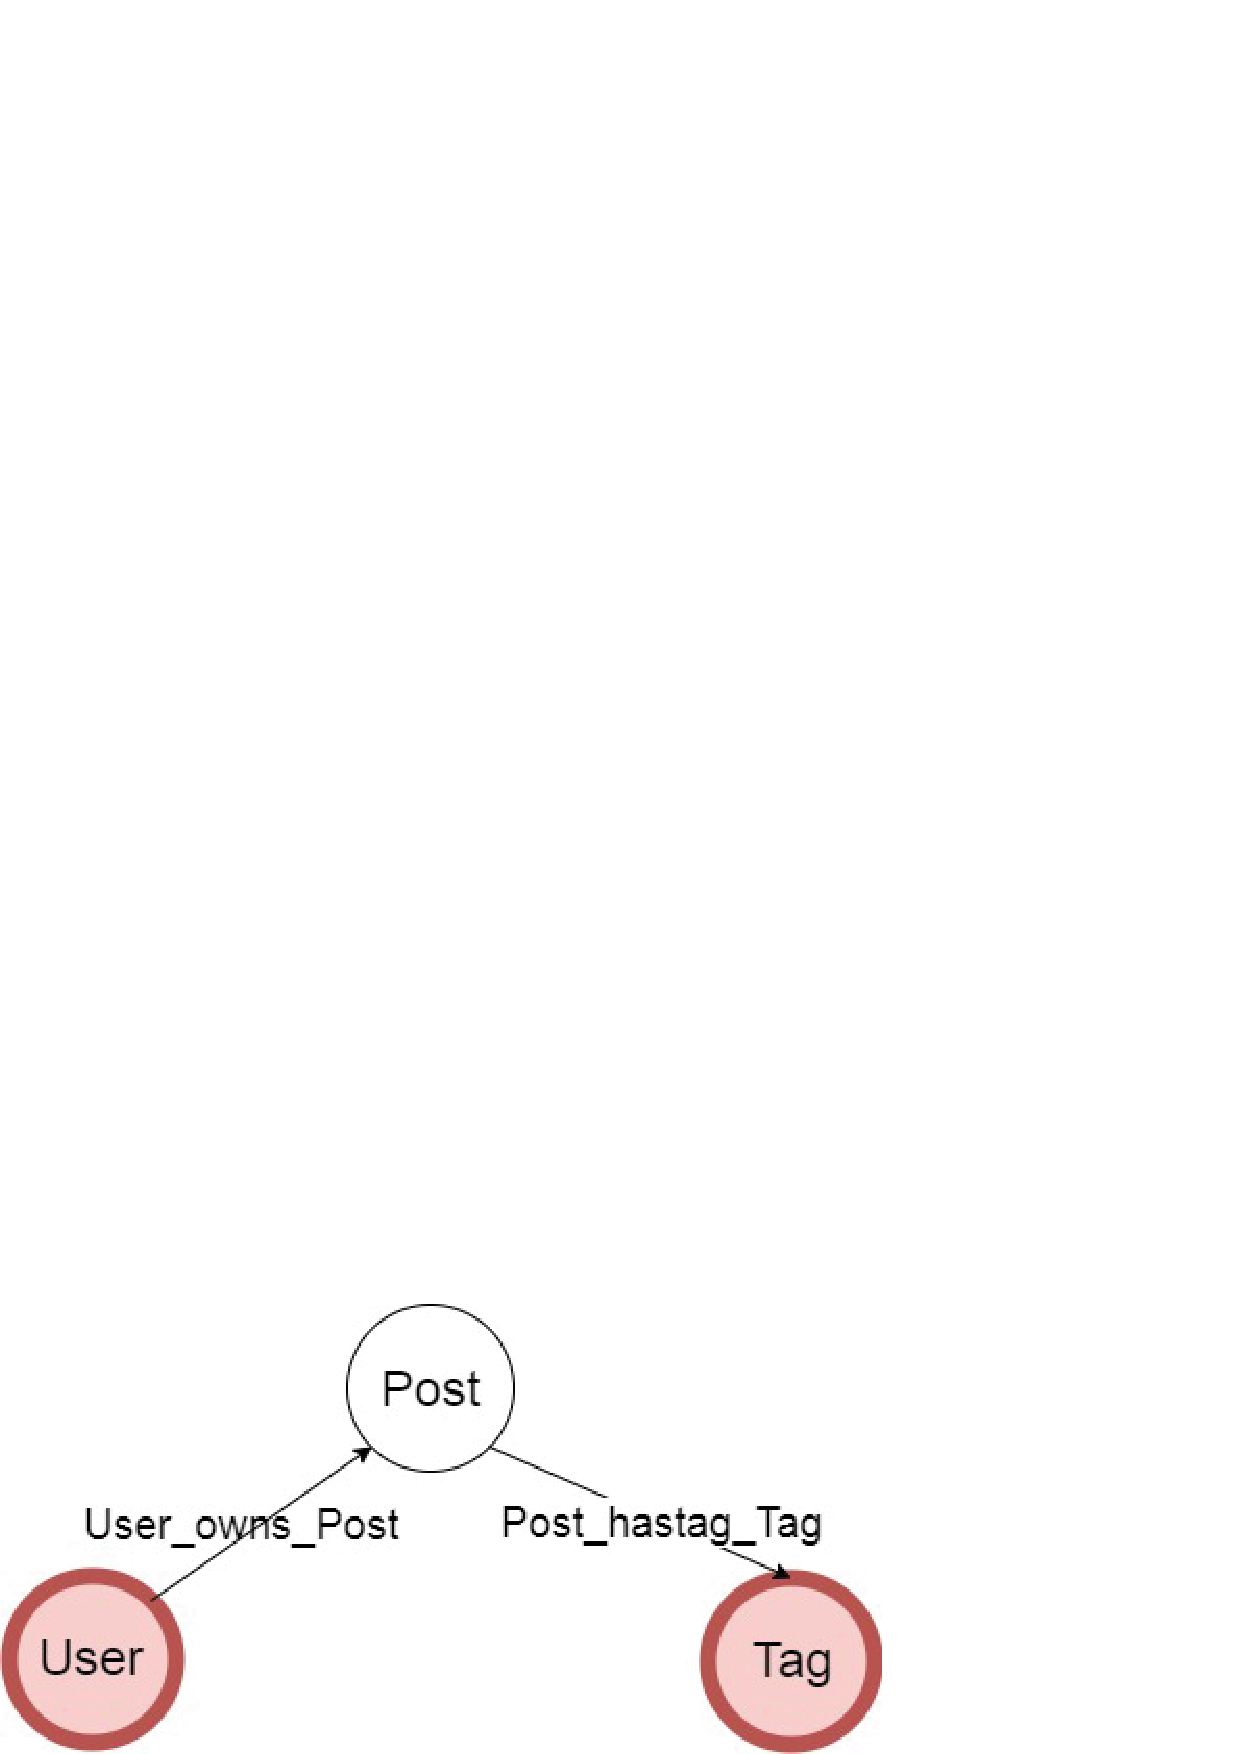
\includegraphics[scale=0.35]{pic/bordernode.pdf}
	\caption{``Border nodes'' of structure \textit{User-Post, Post-Tag}.}
	\label{border node}
\end{figure}
\end{itemize}


We use Policy \#1 in our implementation. However if keeping IDs of inner nodes and edges overwhelmingly increases result length, it's wise to choose Policy \#2 as space cost becomes too high.

For properties, we consider the following two policies.

\begin{itemize}
\item Policy \#1 keeps all properties.
\item Policy \#2 only keeps properties that were queried in previous workloads.
\end{itemize}

Our suggestion is to consider the proportion of properties which were queried in previous workload over all properties in the data schema. For example, in our experiment only a small proportion of properties were queried. We choose Policy \#2 as it is a waste of space to keep all properties.

%\intodo{Please add a short section discussing how to update the materialized views. For example, along the execution of more and more queries, there could be change of ``hot structures''. How we update the materialized views, or possible solutions to address this problem.}

%----------------------------------------------------------------------
\subsection{Update on Materialized Views}
%----------------------------------------------------------------------
The solution we have discussed so far is applicable for static scenarios (with fixed previous workload). We now expand our solution to dynamic scenarios: as queries are executed, there could be change of ``hot structures'' and ``properties of interest''. Thus updates on materialized views are necessary. Remember that we have a memory budget, therefore in some cases obsolete materialized views need to be swapped out for new ones. To achieve this, we maintain a sliding window over previous queries. After executing a certain number of queries, we perform materialized view selection over only ``recent queries'' which are in the sliding window. Old views that need to be swapped out are eliminated by simply releasing their memory. For newly selected views we materialize them. For old views that do not need to be swapped out, we do nothing as they are already materialized in memory. In this way periodical update on materialized views can be realized.


%----------------------------------------------------------------------
\section{Query Processing}
\label{Future Query Processing Part}
%----------------------------------------------------------------------
Query processing aims at processing incoming queries efficiently using materialized substructures and cuboids. When a query $q$ arrives, we first consult materialized cuboids. If $q$ can be answered with an aggregation over any materialized cuboid, we select the cuboid with the minimum space and directly scan over it to produce result of $q$. If $q$ cannot be answered by any cuboid, we decompose $q$ and use substructures as much as possible to compute the result of $q$.

\begin{algorithm}[H]
\label{alg:Query Processing}
\caption{Query Processing}
\LinesNumbered
\textbf{System:} $C$: a set of materialized cuboids\\ $S$: a set of materialized substructures\\
\KwIn{$q$: a query\\}
\KwOut{$r$: result of $q$}

$minspace\leftarrow \infty $\;
mincuboid \leftarrow NULL\;
\ForEach{$cuboid \in C$}{
	\If{cuboid.structure = q.structure and q.dimension $\subseteq$ cuboid.dimension}{
		\If{$cuboid.space<minspace$}{
			minspace \leftarrow cuboid.space\;
			mincuboid \leftarrow cuboid\;
		}
	}
	
	\eIf{$mincuboid \not= NULL$}{
		$r \leftarrow aggregate(mincuboid, q)$\;
	}{
		$r \leftarrow Decompose\_Join(q)$\;
	}
}
\end{algorithm}
%\clearpage

Algorithm \ref{alg:Query Processing} describes the generic work flow of query processing. Given an incoming query $q$,
we first look up materialized cuboids and find if any cuboid can be used to answer $q$ (lines 4-9). Note that $cuboid.space$ in line 5 was computed in line 9 in Algorithm \ref{alg:SingleCubePlanner}. Then, we check if $q$ can be answered by cuboid materialization. If so, we perform aggregation operation over the cuboid (line 11). Otherwise, we need to decompose $q$ into substructures and compose the result (line 13). Function $aggregate(mincuboid, q)$ is the classic aggregation operation. We will discuss how function $Decompose\_Join(q)$ is implemented at the end of this section.

%----------------------------------------------------------------------
\subsection{Substructure Selection}
\label{Substructure Selection}
%----------------------------------------------------------------------

Before discussion on $Decompose\_Join(q)$, we need to first solve a ``Substructure Selection'' problem. In order to decompose a query $q$, we need to consider which materialized substructures we need to use. We need to make decision when candidate substructures in $S$ overlap. For example suppose $q$ has structure \textit{Badge-User, User-Post, Post-Tag}.

And S consists of substructures

(1) Badge-User

(2) Badge-User, User-Post

(3) User-Post, Post-Tag

(4) Post-Tag

(5) User-Post.

We can get structure of $q$ by joining structures of (1) and (3). Thus (1) and (3) seem to be a possible combination for substructure selection in this case. Actually we may have at least three possible substructure selections: (1) and (3); (2) and (4);
(1), (4) and (5). The key question is which selection will result in fastest processing time on $q$? Here are some intuitions to solve this tricky question. First, when we select substructures one by one, we do not select a substructure when it is covered by selected substructures. For example we will not consider (1) if (2) has been selected as (1) is covered by (2). Second, we prefer to minimize total size of selected substructures as we need to at least access each selected view once. We prefer less memory access. Third, we prefer smaller number of selected substructures as intuitively this causes less times of joins.

We propose a greedy algorithm for substructure selection based on user defined heuristics. Users may define heuristic functions based on intuitions (like the three intuitions mentioned above). The idea of the greedy algorithm is to always pick up next substructure with highest score of user defined heuristic function $h(s)$, which returns heuristic score for a substructure $s$. Some example heuristics are \#edges of substructure, score calculated in StructurePlanner (Line 11 in Algorithm \ref{alg:StructurePlanner}), table size etc.

\begin{algorithm}[H]
\caption{SelectSubstrucre}
\label{alg:SelectSubstrucre}
\LinesNumbered
\textbf{System:} $S$: a collection of materialized substructures\\ $h(s)$: user defined function. It returns the heuristic score of a substructure $s$.\\
\KwIn{$q$: a future query\\}
\KwOut{$V$ : selected views for future joining\\ $uncoveredStruc$: structure not covered by selected views\\$uncoveredProp$: properties not covered by selected views\\}
uncoveredStruc \leftarrow q.structure\;
uncoveredProp\leftarrow q.properties\;
$coveredStruc\leftarrow \emptyset$\;
$V\leftarrow\emptyset $\;
\ForEach{$s \in S$ ordered by h(s)}{
	\If{s $\subseteq$ uncoveredStruc and s $\not\subseteq$ coveredStruc}{
		$V \leftarrow V \cup \{s\}$\;
		$coverdStruc \leftarrow coveredStruc \cup s.structure$\;
		uncoveredStruc \leftarrow uncoveredStruc - s.structure\;
		uncoveredProp \leftarrow uncoveredProp -s.properties\;
	}
}
\end{algorithm}
%\clearpage

Lines 1-2 initialize $uncoveredStruc$ and $uncoveredProp$, which keeps track of structures and properties which have not been covered by selected substructures. Such uncovered structures and properties will need to be fetched from the database. Line 3 initializes $coveredStruc$, which keeps union of selected substructures. Line 5 starts iteration over substructures ordered by user-defined heuristics $h(s)$. Line 6 assures that a candidate substructure that is totally covered by selected substructures will be disqualified. In the above example, suppose we have already selected (2), there is no need to select (1) since (1) is totally covered by (2).

%----------------------------------------------------------------------
\subsection{Decomposition and Join}
\label{Query Decomposition}
%----------------------------------------------------------------------
In this section, we  discuss how to implement function $Decompose\_Join(q)$ (as in Algorithm FutureQueryProcessing in subsection \ref{Future Query Processing Part}). Besides $Decompose\_Join(q)$, we shall discuss two other variations of implementation: $Decompose\_Join^{*}$ and $Decompose\_Join^{+}$.

%----------------------------------------------------------------------
\subsubsection{\#1 $Decompose\_Join$}
%----------------------------------------------------------------------
Given a query $q$, we use the previously discussed algorithm ``SelectSubstrucre'' to select a set of substructure materializations $V$. However, substructures in $V$ may not completely cover the structure of $V$. If there is any remaining structure ($uncoveredStruc$) and properties ($uncoveredProp$) that $V$ does not cover, we need to retrieve them from the database. We call such remaining structures and properties fetched from the database ``complementary  components''. After all these components (both materializations and ``complementary  components'') are finally ready, we join and aggregate them to produce final results.

\begin{algorithm}[H]
\caption{Decompose\_Join}
\LinesNumbered
\textbf{System:} $S$: a collection of materialized substructures\\
\KwIn{$q$: a future query\\}
\KwOut{$r$: result of $q$}
$\Sigma \gets \emptyset $\;
$V, uncoveredStruc, uncoveredProp \gets SelectSubstrucre(q) $\;
$\Sigma \gets \Sigma \cup V $\;
$Splits\leftarrowsplit(uncoveredStruc, uncoveredProp)$\;
\ForEach{s: Splits}{
	$\Sigma \gets \Sigma \cup \{retrieve(s)\} $\;
}
$r \leftarrow join\_aggregate(\Sigma, q)$\;
\end{algorithm}

Line 1 initializes $\Sigma$, which maintains a set of all components (materializations and ``complementary  components'') that are needed. Line 2 selects substructures using SelectSubstructure algorithm. $uncoveredStruc$ and $uncoveredProp$ refer to structures and properties which are not covered by selected substructures. They are ``complementary components'' and will be retrieved from database servers. Line 4 splits $uncoveredStruc$ and $uncoveredProp$ into connected components. We retrieve each connected component from the database server. Note that splitting is necessary since $uncoveredStruc$ may not be exactly one connected component. Line 8 joins and aggregates all materials together to produce results.

Function \textit{split(uncoveredStruc, uncoveredProp)} is implemented by a classic connected components detection algorithm. It splits $uncoveredStruc$ and $uncoveredProp$ into connected components (structures). We want to retrieve each connected structure separately from the database because otherwise it may result in unnecessarily large results of Cartesian products of several disconnected structures. Function \textit{$materialize(s)$} retrieve ``complementary components'' $s$ from the database server. Function \textit{join($\Sigma$, q)} join tables of $\Sigma$ together and aggregate over properties based on $q$. Joins over multiple tables is a well-studied topic. Joining order and join technique (hash join etc.) are two important aspects of this topic. In our implementation we use hash join and our joining order policy is to keep joining two tables which have minimum sum of table sizes and have common column(s). That is, we tend to select two smaller tables to join.

%----------------------------------------------------------------------
\subsubsection{\#2 $Decompose\_Join^{*}$}
%----------------------------------------------------------------------
$Decompose\_Join$ retrieve ``complementary components'' from the database in a naive manner. We adopt the idea of Semi-Join \cite{DBLP:journals/dr/Ozsoyoglu99} and propose another way of implementation: $Decompose\_Join^{*}$. Semi-join takes advantage of ``selection effect'' of natural joins. In $Decompose\_Join^{*}$, we first perform joins over substructures of $V$ even before fetching ``complementary components'' from the database. Line 3 performs $join(V)$ before $retrieve$ in Line 7. We call this phase ``first round of joins''.  Note that substructures in $V$ may reside in multiple connected components. Thus $V^{*}$ may consist of multiple intermediate tables. The purpose for first round of joins is that it provides ``candidate'' node and edge IDs for future joins (thanks to `selection effect'' of natural joins). When fetching ``complementary components'' from the database server, we inform database server such candidate node and edge IDs so that search space for ``complementary components'' is narrowed down ($retrieve^{*}(s, V^{*})$ in Line 7). We name this approach $Decompose\_Join^{*}$.

\begin{algorithm}[H]
\caption{$Decompose\_Join^{*}$}
\LinesNumbered
\textbf{System:} $S$: a collection of materialized substructures\\
\KwIn{$q$: a future query\\}
\KwOut{$r$: result of $q$}
$\Sigma \gets \emptyset $\;
$V, uncoveredStruc, uncoveredProp \gets SelectSubstrucre(q) $\;
$V^{*}\leftarrowjoin(V)$\;
$\Sigma \gets \Sigma \cup V $\;
$Splits\leftarrowsplit(uncoveredStruc, uncoveredProp)$\;
\ForEach{s: Splits}{
	$\Sigma \gets \Sigma \cup \{retrieve^{*}(s, V^{*})\} $\;
}
$r \leftarrow join\_aggregate(\Sigma, q)$\;
\end{algorithm}
%\clearpage


We explain implementation of function $retrieve^{*}(s, V^{*})$. It fetches results from the database by passing candidate IDs information (from join result $V^{*}$). Syntax to achieve this varies by database. In SQL and Cypher we may pass candidate IDs using a ``WHERE'' statement. Besides Neo4j driver supports passing lists of integers as arguments in a query.


We compare $Decompose\_Join^{*}$ vs.  $Decompose\_Join$ and summarize following pros and cons of $Decompose\_Join^{*}$. $Decompose\_Join^{*}$ helps accelerate retrieval process from back end databases in two aspects. First, since screened out candidate IDs are provided, database back end only needs to iterate through a portion of nodes and edges. This saves database processing time. Second, candidate IDs have a ``selection'' effect thus size of retrieval results is deducted. Thus time caused by result transmission will be reduced. The disadvantages are twofold. First, $Decompose\_Join^{*}$ has to transmit IDs. Second,  $Decompose\_Join^{*}$ performs two rounds of join; first on $V$ before ``complementary components'' are ready,  followed by second round of joins. In terms of optimization on join orders, $Decompose\_Join$ is better because its join order is decided over all the tables, whereas in $Decompose\_Join^{*}$ tables are separated by two rounds of joins, which narrows down the scope of all possible join orders.

------------------
\subsubsection{\#3 $Decompose\_Join^{+}$}
%----------------------------------------------------------------------
We mentioned two advantages of $retrieve^{*}(s, V^{*})$. However a disadvantage of $retrieve^{*}(s, V^{*})$ is an overhead of transmission of candidate IDs. We propose a decisive way to evaluate the trade-off between overhead and benefits of $retrieve^{*}(s, V^{*})$ and choose between $retrieve^{*}(s, V^{*})$ and $retrieve(s)$. $Decompose\_Join^{+}$ is derived from $Decompose\_Join^{*}$. The trick is to revise Line 7 by using $decide(s,V^{*})$ to choose the better way between $retrieve^{*}(s, V^{*})$ and $retrieve(s)$.

\begin{algorithm}[H]
\caption{$Decompose\_Join^{+}$}
\LinesNumbered
\textbf{System:} $S$: a collection of materialized substructures\\
\KwIn{$q$: a future query\\}
\KwOut{$r$: result of $q$}
$\Sigma \gets \emptyset $\;
$V, uncoveredStruc, uncoveredProp \gets SelectSubstrucre(q) $\;
$V^{*}\leftarrowjoin(V)$\;
$\Sigma \gets \Sigma \cup V $\;
Splits\leftarrowsplit(uncoveredStruc, uncoveredProp)\;
\ForEach{s: Splits}{
	\eIf{decide(s,$V^{*}$)}{
		$\Sigma \gets \Sigma \cup \{retrieve^{*}(s, V^{*})\} $\;
	}{
		$\Sigma \gets \Sigma \cup \{retrieve(s)\} $\;
	}
}
$r \leftarrow join\_aggregate(\Sigma, q)$\;
\end{algorithm}
%\clearpage

Implementation of function $decide(s,V^{*})$ is detailed as follows. We first estimate result sizes of the two retrieval methods: $retrieve^{*}(s, V^{*}).estSize$ and $retrieve(s).estSize$. $retrieve(s).estSize$ can be returned by $space(substructure)$ in Algorithm \ref{alg:StructurePlanner}. The tricky one is $retrieve^{*}(s, V^{*}).estSize$, whcih we estimate as follows:
\begin{enumerate}
\item  Randomly sample a small number of candidate IDs.

\item  Execute $retrieve^{*}$ but pass only sampled candidate IDs in (1). We call this a ``trial query''. We want to use the ``trial query'' to estimate result length of actual $retrieve^{*}(s, V^{*})$. Since we only pass a small number of IDs, time cost of ``trial query'' is acceptably small.

\item  Calculate $retrieve^{*}(s, V^{*}).estSize$ proportionally using the result of ``trial query''.
\end{enumerate}
\par
We compare $retrieve^{*}$'s benefit in result size reduction against its cost in passing candidate IDs by evaluating $(retrieve(s).estSize - retrieve^{*}(s, V^{*}).estSize) / sizeOf(candidateIDs)$ and compare the ratio with a threshold $\gamma$ and make a decision. $\gamma$ is important as it directly affects decision making. We suggest running some prior tests in order to adjust $\gamma$ to a proper value. The prior tests are conducted by executing some sample queries by both $Decompose\_Join$ and $Decompose\_Join^{*}$. In each test, the value of $(retrieve(s).estSize - retrieve^{*}(s, V^{*}).estSize) / sizeOf(candidateIDs)$, together with correct decision between $Decompose\_Join$ and $Decompose\_Join^{*}$ (the one with less processing time) are recorded. We view it as a binary classification problem and  it can be easily solved by linear regression.   

We compare  $Decompose\_Join^{+}$ vs $Decompose\_Join^{*}$: We see that $Decompose\_Join^{+}$ performs two rounds of joins like $Decompose\_Join^{*}$. The major difference is that $Decompose\_Join^{+}$ plays ``trial query''. The principle behind ``trial query'' is to pay an acceptable price to make a wise decision on ``complementary components'' retrieval. Our experiments show that a good decision making on ``complementary components'' retrieval saves much more time than the time cost of ``trial queries'', results and discussion of which will be presented in next chapter.




%----------------------------------------------------------------------



%======================================================================
\chapter{Experiments}
%======================================================================

%----------------------------------------------------------------------
\section{Experiment Setup}
%----------------------------------------------------------------------

%Our main focus is to evaluate different strategies for preprocessing and query evaluation. For instance, the threshold of “Is hot-structure” part in the diagram,  selection policy for materialized substructures in “Cube-Planner” and “Structure-Planner” , different heuristics when ranking sub-structures during decomposition in “Decomposition and Joining” etc.

There are two purposes of our experiments. First, to compare query processing efficiency of our system with naive Neo4j system. Second, to test how different settings (of parameters and choices of strategies) in our solution affect query processing efficency. Experiments were run on a same set of queries on a same dataset. For datasets, we chose to use real-world datasets. As For queries, we wrote queries with real meanings instead of generating random queries. 

%----------------------------------------------------------------------
\subsection{Datasets}
%----------------------------------------------------------------------

We used a StackOverFlow dataset in our experiment. We created this dataset using raw information from https://archive.org/details/stackexchange. The dataset contains user-contributed content (such as user information, posts etc) on www.stackoverflow.com. The dataset contains 10 different node labels and 12 different edge labels.  Figure \ref{fig:5:1} shows a meta graph of 7 nodes and 8 edges which were involved in our experiments. StackOverFlow dataset is a large dataset which contains over 300 million nodes and more than 400 million edges. Its size on hard disk is 44.5GB. 

\begin{figure}[H]
	\centering
	\includegraphics[scale=0.5]{pic/MetaGraphExperiment (1).jpg}
	\caption{A meta graph of StackOverFlow dataset.}
	\label{fig:5:1}
\end{figure}  


%----------------------------------------------------------------------
\subsection{Query Workloads}
%----------------------------------------------------------------------
24 queries of real meanings were written into a query pool. We randomly selected 12 queries as previous workload, leaving the rest 12 ones as future workload. Queries are listed below.


\\\textbf{Previous WorkLoad:}

User-Post: User.UpVotes, Post.Score=10

User-Post: User.UpVotes, (AVG)Post.Score

User-Post: User.Age, (SUM)Post.ActiveMonth

User-Post: User.CreationDate_Year, Post.PostTypeId=1

Badge-User, User-Post, Post-Tag: Tag.TagName, User.CreationDate_Year=2017

Badge-User, User-Post, Post-Tag: Tag.TagName, Badge.Name

Badge-User, User-Post:Badge.Date_Year,(AVG)Post.Score

Badge-User, User-Post:Badge.Class,(AVG)Post.ActiveMonth

User-Post, Post-Tag: (AVG)User.Age, Tag.TagName

User-Post, Post-Tag: (AVG)User.UpVotes, Tag.TagName=Java

User-Post, Post-Vote: (AVG)User.UpVotes, Vote.VoteTypeId

Post-Comment, Post-PostHistory: PostHistory.PostHistoryTypeId=5, (AVG)Comment.Score


\\\textbf{Future WorkLoad:}

User-Post: User.CreationDate_Year=2017, Post.PostTypeId

User-Post: (AVG)User.UpVotes,Post.Score

User-Post: Post.ActiveMonth, (AVG)User.Age

User-Post: User.CreationDate_Year

Badge-User, User-Post, Post-Tag: Tag.TagName, Badge.Class

Badge-User, User-Post, Post-Tag: Tag.TagName, Badge.Date_Year

Badge-User, User-Post:Badge.Name, Post.PostTypeId

User-Post, Post-Tag: User.UpVotes, Tag.TagName, Post.PostTypeId=2

User-Post, Post-Tag:User.CreationDate_Year, Tag.TagName

Post-PostLink, Post-Tag: Tag.TagName=database, PostLink.LinkTypeId

Badge-User, User-Comment: Badge.Class, (AVG)Comment.Score

Post-Tag, Post-Vote: Tag.TagName




%----------------------------------------------------------------------
\subsection{System Setting}
%----------------------------------------------------------------------

We ran all the experiments on a Linux cluster machine with main memory of 256GB. Our system is implemented in Java. We set initial Java vitual machine memory as 100GB and maximum Java vitual machine memory as 200GB.

%----------------------------------------------------------------------
\subsection{Neo4j Configuration}
%----------------------------------------------------------------------
We used Neo4j Community v3.1.3 as database server. Neo4j's initial memeroy size is set as 60GB and maximum memeroy size as 200GB. We used Neo4j's official Java driver to interact with Neo4j server.

%----------------------------------------------------------------------
\section{Aspects of Interest}
\label{Aspects of Interest}
%----------------------------------------------------------------------

As we mentioned, there are two purposes of our experiments. The second purpose requires tests on how different settings in our system affect query processing efficency. We list the following aspects of interest which were tested. Default setting for each aspect is also presented. For variable control purpose, in each test all aspects were set to default settings, except for the only one aspect on which we would test.  

\textbf{Materialization}
\begin{itemize}

\item  Memory limit, i.e. $\sigma$ in Algorithem \ref{alg:StructurePlanner}. Default setting: 6GB.

\item  Algorithm in materialized view selection \ref{Materialization Part}. For cuboid selection, we  campared CubePlanner \ref{sec:CubePlanner} with ``Patial Materialization'' algorithm (PMA) proposed in Graph Cube \cite{DBLP:conf/sigmod/ZhaoLXH11}. For substructure selection we will compared StructurePlanner \ref{Structure Planner} with frequent pattern mining algorithm (FPM). Default setting: CubePlanner and StructurePlanner.

\item Frequency threshold for identification of “hot structures”, i.e. $\omega$ in Algorithm \ref{alg:1}. Default setting: 4. Section \ref{Frequency Threshold} explains why setting $\omega$ as 4. 

\item Storage for merialized views. We will compare main memory storage v.s. hard disk storage. Default setting: main memory storage.

\end{itemize}

\textbf{Future Query Processing}
\begin{itemize}
\item  Choice of score functions in ranking substructures during ``Substructure Selection'' \ref{Substructure Selection}, i.e. $h(s)$ in Algorithm \ref{alg:SelectSubstrucre}. Default setting: $h(s)$ returns the score of $s$ calculated in StructurePlanner (as result of line 11 in Algorithm \ref{alg:StructurePlanner}). 

\item  Choice among using $Decompose\_Join$, $Decompose\_Join^{*}$ and $Decompose\_Join^{+}$ in ``Decomposition and Join'' \ref{Query Decomposition}. Default setting: $Decompose\_Join$.

\end{itemize}

Besides, we also ran experiments on the smaller dataset to see how performance varies in datasets of different sizes.  

%----------------------------------------------------------------------
\section{Results and Discussion}
\label{Results and Discussion}
%----------------------------------------------------------------------
In this section, results of experiments are presented and explainations of results are given. 

%----------------------------------------------------------------------
\subsection{Our System vs. Neo4j Baseline}
%----------------------------------------------------------------------
We used default settings for our system and compared  with naive Neo4j system over processing time for the future workload (12 queries).


\begin{figure}[H]
	\centering
	\includegraphics[scale=0.5, angle=270]{plot/neo4j}
	\caption{Processing time for future workload by our proposed solution v.s. Neo4j.}
	\label{fig:neo4j}
\end{figure}

Figure \ref{fig:neo4j} shows processing time for 12 future queries by both our system and Neo4j. We see that with a cost of 5.7GB materializd view storage, which is acceptable considering size of the dataset, our solution achieved remarkable efficiency improvement.

\begin{figure}[H]
	\centering
	\includegraphics[scale=0.5]{"pic/MetaGraphExperiment_Hot (1)"}
	\caption{Substructure selected by StructurePlanner.}
	\label{fig:metagraphexperimenthot}
\end{figure}

We detail how our system worked. First, \textit{User-Post} was identified as ``hot structure''. As a result, P1 - P4 were passed to CubePlanner and P5 - P12 were passed to StructurePlanner. Cuboids selected by CubePlanner are \textit{User-Post: User.Age, Post.ActiveMonth}; \textit{User-Post: User.CreationDate\_Year, Post.PostTypeId}; \textit{User-Post: User.UpVotes, Post.Score}. Figure \ref{fig:metagraphexperimenthot} highlights substructures S that StructurePlanner selected:  \textit{User-Post} (s1), \textit{Post-Tag} (s2) and \textit{Badge-User} (s3). From observation of previous workload, we can tell that StructurePlanner made a wise decision as these three substructures are able to cover most of previous queries. 

We give explainations on performance differences by each query. Avarage improvement rate for Q1 - Q4 is around 7000. This is because Q1 - Q4 got hit by C (``cuboid hit''). As a result processing time is reduced to a much greater extent than Q5 - Q12 (which did not get ``cuboid hit''). Note that time complexities of cuiboid aggregation and substructure joins are in different scales. Time complexity of cuiboid aggregation is bounded by production of cardinalities of involved properties. When it comes to substructure joins, however, time complexity is related to the actual data sizes. Q5 - Q9 are totally covered by S. As a result no ``complementary components'' were fetched from database.  Q10 - Q12 are partially coverd by S.  ``Complementary components'' were fetched from database, which increased time cost. As a result improvement rate for Q5 - Q9 ranges from around 10 to more than 30, while improvement rate for Q10 - Q12 ranges around 10, which is lower. To conclude, our system greatly improved query processing efficency. Improvement rates vary in different senerios of cuboid and structure ``hits''.




%----------------------------------------------------------------------
\subsection{Frequency Threshold}
\label{Frequency Threshold}
%----------------------------------------------------------------------
Frequency threshold $\omega$ has an important effect on query processing efficiency. A change of $\omega$ may result in changes of ``hot structures'', followed by changes in inputs for CubePlanner and StructurePlanner. This will further result in different materialized view selection and finally different query processing performance. As indicated in Section \ref{Overview of Materialization Part}, $\omega$ serves as a minimum bar to convince that building a cuiboid over a ``hot structures'' is worthy (``cuboid hit'' assured). We think 4 is an appropritate choice for $\omega$ in our test case considering frequency count of structures in previous workload (as shown in the below table). 

\begin{center}
	\begin{tabular}{ | c | c |}  
		\hline
		Structure	&Frequency	\\ \hline 
		\textbf{User-Post} 	&\textbf{4} \\ \hline
		Badge-User, User-Post, Post-Tag 	&2 \\ \hline
		Badge-User, User-Post	&2 \\ \hline
		User-Post, Post-Vote	&2 \\ \hline
		Badge-User, User-Comment	&1 \\ \hline
		Post-Comment, Post-Vote	&1 \\ \hline
	\end{tabular}
	\end {center}

Suppose we lower $\omega$ to 2. \textit{Badge-User, User-Post, Post-Tag} will be ``hot structure''. As a result, cuboid selection over \textit{Badge-User, User-Post, Post-Tag} will be considered based on merely two queries (P5 and P6). Notice that Q5 and Q6, which have structure \textit{Badge-User, User-Post, Post-Tag}, will never get ``cuboid hit''. This is because properties Badge-Class in Q5 and Badge-Date_Year in Q6 did not even appear in P5 and P6. That is to say, in this case any cuboid selected over \textit{Badge-User, User-Post, Post-Tag} will be useless. In addtion, when $\omega$ is set to 2, input for StructurePlanner will be only two queries (Q11 and Q12). Note that structure frequency counts of these two queries are both 1. In other word, these are the most ``random'' queries. Note that the idea of StructurePlanner is discovery of useful substructures based on a sufficent number of ``less hot'' queries. In this case two ``random'' queries is not an ideal input for StructurePlanner.  

On the other side, suppose we increase $\omega$ to 5, then there will be no cuboid materialized. As a result Q1 - Q4 will be processed using substructure materialization (s1). Despite this is still faster than naive Neo4j system, the outstanding improvement rate of ``cuboid hit'' cannot be achieved. 

Figure \ref{fig:omega} presents total processing time under different settings of $\omega$. We reach our conclustion that $\omega$ did have a significant effect over system performance. Actually determination on the value of $\omega$ is an interesting classification problem (based on frequency count). However we will leave this topic to future work since it is not the main focus of our work. 

\begin{figure}[H]
	\centering
	\includegraphics[scale=0.5, angle=270]{plot/omega}
	\caption{Total processing time under different settings of $\omega$.}
	\label{fig:omega}
\end{figure}


%----------------------------------------------------------------------
\subsection{Space Cost Limit}
%----------------------------------------------------------------------
Our default setting \ref{Aspects of Interest} sets space cost limit for materialized views $\sigma$ to be 6GB and the actual space cost of materialized views is 5.7GB. If we change $\sigma$ we may get different materialized views thereby different efficiency performance. Figure \ref{fig:limit} shows how total processing time varied by different actual space costs (which were caused by setting $\sigma$ to 6GB, 4GB and 2.5GB). From the figure we see that with more views being materialized, total processing time is reduced. However the maginal effect from new views decreased as more views were materialized. This indicates that our Greedy Selection Framework successfully picked candidates by their maginal benefits.

\begin{figure}[H]
	\centering
	\includegraphics[scale=0.5, angle=270]{plot/limit.eps}
	\caption{Efficiency v.s. Space Cost}
	\label{fig:limit}
\end{figure}

%----------------------------------------------------------------------
\subsection{Storage for Merialized Views}
%----------------------------------------------------------------------
In the default setting \ref{Aspects of Interest}, materialized views are stored as objects in main memory. This provides fast access to the views but causes a main memory storage cost. Alternatively materialized views can be serialized and stored as files on hard disks. Figure \ref{fig:disk} shows that hard disk storage did not perform as fast as main memory storage, but the drop in efficency is acceptable. Such drop in efficency is owing to I/0 overhead in reading materialized views from files.

 One interesting question is since eventually materialized views are be read into main memory, what is the point of storing them in files? Our answer is that in cases when main memory is far too small for holding all selected views, hard disk materialization provides a lower level of storage of sufficent volume.
 
\begin{figure}[H]
	\centering
	\includegraphics[scale=0.5, angle=270]{plot/disk}
	\caption{Main memory storage v.s. hard disk storage}
	\label{fig:disk}
\end{figure}

%----------------------------------------------------------------------
\subsection{CubePlanner v.s. PMA}
%----------------------------------------------------------------------
We compared CubePlanner \ref{CubePlanner} in our solution with PMA in Graph Cube \cite{DBLP:conf/sigmod/ZhaoLXH11}. Figure \ref{} and \ref{} show that CubePlanner outperformed PMA in both query processing efficency and space cost. 

Acutally both two approaches are considered as implementations of Greedy Selection Framework \ref{s:Greedy Selection Framework}. We reveal differences between the two implementations. CubePlanner uses the ratio of marginal benefit over space cost as a score for candidate ranking (line 11 inAlgorithm \ref{alg:SingleCubePlanner}). While PMA only considers maginal benefit. That is to say, space cost does not count in PMA. This gives rise to why CubePlanner outperformed PMA in terms of space cost. Moreover, PMA treats each combination of properties with equal weight, regardless of how many times a combination appeared in previous queries. For example in our test case, combination of {User.UpVotes, Post.Score} appeared twice in previous workload. But PMA would treat {User.UpVotes, Post.Score} with the same weight as those combinations that were not even queried in previous workload (\{User.UpVotes, Post.PostTypeId\} etc). As a result, CubePlanner adopted more information from previous workload and thus made better selection. 

%----------------------------------------------------------------------
\subsection{StructurePlanner v.s. FPM}
%----------------------------------------------------------------------
We compare our algorithm \ref{alg:StructurePlanner} in StructurePlanner with FPM. In FPM we set minimum support to 2 considering frequency count as listed in the table in Section \ref{Frequency Threshold}. These two ways provided different substrcutre selections which led to different processing performance. Figure \ref{fig:fpm} and \ref{fig:fpmspace} show that our StructurePlanner outperformed FPM in both efficency performance and space cost.

\begin{figure}[H]
	\centering
	\includegraphics[scale=0.5, angle=270]{plot/fpm}
	\caption{Total processing time: StructurePlanner v.s. FPM}
	\label{fig:fpm}
\end{figure}

\begin{figure}[H]
	\centering
	\includegraphics[scale=0.5, angle=270]{plot/fpm_space}
	\caption{Space cost: StructurePlanner v.s. FPM}
	\label{fig:fpmspace}
\end{figure}

Figure \ref{fig:metagraphexperimenthot} highlights three selected substructures by StructurePlanner. As mentioned it is a wise selection as these three substructures were able to cover the most of previous queries. However, Frequent Pattern Mining selected \textit{Badge-User, User-Post, Post-Tag}. This is a bad selection because it was useful only for Q5 and Q6. In addition, materialization of \textit{Badge-User, User-Post, Post-Tag} results in even more space cost than materialization of the three edges seperately (as selected by StructurePlanner). Figure \ref{fig:qfpm} details processing time for each query. FPM only outperformed StructurePlanner on Q5 and Q6. This is because by FPM Q5 and Q6 were processed by direct aggreagation over structure materialization of \textit{Badge-User, User-Post, Post-Tag}, while by StructurePlanner table joins of s1, s2 and s3 was required, which costed more time. However for Q7 - Q12, StructurePlanner outperformed as it got at least patial ``substructure cover'' while selected result of FPM helped nothing.

\begin{figure}[H]
	\centering
	\includegraphics[scale=0.5, angle=270]{plot/qfpm}
	\caption{Processing time for each query: StructurePlanner v.s. FPM}
	\label{fig:qfpm}
\end{figure}


%----------------------------------------------------------------------
\subsection{Substructure Selection}
%----------------------------------------------------------------------

In our experiment, $h(s)$ in Algorithm \ref{alg:SelectSubstrucre} did not make any difference during ``Substructure Selection'' \ref{Substructure Selection}. This is because the three selected substructures do not share any common edge. Note that senerios in Section \ref{Substructure Selection} where multiple valid combinations of materialized substructures exist only happen when materialized substructures have overlaps. 

%----------------------------------------------------------------------
\subsection{Decompose\_Join}
%----------------------------------------------------------------------
We conducted tests on $Decompose\_Join$, $Decompose\_Join^{*}$ and $Decompose\_Join^{+}$ in ``Decomposition and Join'' \ref{Query Decomposition}. Such three different implementations in ``Decomposition and Join'' made a difference in processing Q10 - Q12, as they were patially covered by S and fetching ``complementary components'' from Neo4j was needed. Figure \ref{} provides processing time for Q10 - Q12 by the three approaches. $Decompose\_Join^{*}$ performed much better than $Decompose\_Join$ in Q10. This is because $Decompose\_Join^{*}$ passed candidate IDs of posts with ``database'' tag to Neo4j, which provided a tramendous ``filtering effect'' when fetching \textit{Post-PostLink}. As a result, $Decompose\_Join^{*}$'s time for fetching \textit{Post-PostLink} was greatly reduced. Besides, its time for joining \textit{Post-Tag} and \textit{Post-PostLink} also decreased because table sizes of \textit{Post-Tag} and \textit{Post-PostLink} are smaller than those in $Decompose\_Join$ thanks to the ``filtering effect''. This is reflected in Figure \ref{}, from which joining time is seen to have been saved in $Decompose\_Join^{*}$. However $Decompose\_Join^{*}$ performed badly in Q12. This is because ``filtering effect'' of \textit{Post-Tag} in fetching \textit{Post-Vote} is little. In addition, $Decompose\_Join^{*}$ had a considerable overhead of scanning the table of \textit{Post-Tag} in order to get the set of candidate IDs. This explains why $Decompose\_Join^{*}$ took longer time in processing Q12. Figure \ref{} gives total processing time for Q10 - Q12 by the three approaches. We see that $Decompose\_Join^{+}$ had best overall performance. This is because $Decompose\_Join^{+}$ was able to choose the faster approach when fetching ``complementary components'' from Neo4j in senerios like Q10 and Q12 with only a small cost of ``trial query'' \ref{Query Decomposition}. This is reflected in Figure \ref{}. Note that time cost for ``trial query'' is bounded by a constant sampling size (which was set to 100 in our experiments). It is not proportional to actual data size in the dataset. Figure \ref{} shows that time cost ``trial query''is acceptably small. 

To conclude, ``filtering effect'' is an important facter in performance of these three implementations of ``Decomposition and Join''. In general, $Decompose\_Join^{+}$ is the recommended approach as it is able to make the better of the other two approaches with a small cost of ``trial query''.


%----------------------------------------------------------------------
\subsection{Large DataSet v.s. Small DataSet}
%----------------------------------------------------------------------
Besides StackOverFlow dataset (45.8GB), we also tested on a smaller ``StackExchange-Math'' dataset of size 2.57GB. Like StackOverFlow dataset, StackExchange-Math dataset is about a mathematics Q\&A forum (https://math.stackexchange.com).  The raw data of StackExchange-Math dataset also comes from https://archive.org/details/stackexchange and it has exactly the same schema as StackOverFlow dataset. 

Figure \ref{} compares efficiency improvement rate for large dataset and smaller dataset. We see that our system achieved even better performance on larger dataset. 





%======================================================================
\chapter{Conclusion}
%======================================================================
Our work addresses on the urgent need for efficient OLAP processing over large property graphs.  To model the problem mathematically, we provided formal definitions of ``Materialization Selection'', ``Execution Planning'', ``Decomposition Problem'' and ``Composition Problem''. We proposed an end-to-end system to tackle these problems and implemented the system for Neo4j. The main idea of our solution is to accelerate future query processing with materialized views which were selected based on their benefits to previous workload. We conducted experiments on our system and it was proved to be a feasible solution that achieves efficient OLAP queries processing on large graph datasets.   

We summarize future work as follows. First, as reflected in experiment results \ref{Results and Discussion}, efficiency performance of our system is affected by system settings, hence study on appropriate system settings would be a valuable follow-up for our work. Second, the system we implemented so far supports SPARQL like queries over schema graph, instead of data graph. It is realizable to enable processing SPARQL like queries over data graph within our proposed solution framework. The key issue is take isomorphism into consideration during query decomposition and composition. Last but not least, greedy selection framework is with no doubt not a perfect solution for ``Materialization Selection'' problem. We look forward to better solutions for this hard but valuable problem.





%----------------------------------------------------------------------
% END MATERIAL
%----------------------------------------------------------------------

% B I B L I O G R A P H Y
% -----------------------

% The following statement selects the style to use for references.  It controls the sort order of the entries in the bibliography and also the formatting for the in-text labels.
\bibliographystyle{plain}
% This specifies the location of the file containing the bibliographic information.  
% It assumes you're using BibTeX (if not, why not?).
\cleardoublepage % This is needed if the book class is used, to place the anchor in the correct page,
                 % because the bibliography will start on its own page.
                 % Use \clearpage instead if the document class uses the "oneside" argument
\phantomsection  % With hyperref package, enables hyperlinking from the table of contents to bibliography             
% The following statement causes the title "References" to be used for the bibliography section:
\renewcommand*{\bibname}{References}

% Add the References to the Table of Contents
\addcontentsline{toc}{chapter}{\textbf{References}}

\bibliography{uw-ethesis}
% Tip 5: You can create multiple .bib files to organize your references. 
% Just list them all in the \bibliogaphy command, separated by commas (no spaces).

% The following statement causes the specified references to be added to the bibliography% even if they were not 
% cited in the text. The asterisk is a wildcard that causes all entries in the bibliographic database to be included (optional).
\nocite{*}

% The \appendix statement indicates the beginning of the appendices.
\appendix
% Add a title page before the appendices and a line in the Table of Contents
\chapter*{APPENDICES}
\addcontentsline{toc}{chapter}{APPENDICES}
%======================================================================
\chapter[PDF Plots From Matlab]{Meaning for Each Query in Our Experiments}
\label{AppendixA}
% Tip 4: Example of how to get a shorter chapter title for the Table of Contents 
%======================================================================
\section{Previous Workload}
\par
Meaning for each previous query is listed below. 

P1 \hspace{3mm} User-Post: User.UpVotes, Post.Score=9

To see the distribution of users' upvotes for high score (score=9) posts.

P2 \hspace{3mm} User-Post: User.UpVotes, (AVG)Post.Score

To see average post scores by different upvotes. 

P3 \hspace{3mm} User-Post: User.Age, (SUM)Post.ActiveMonth

To see each age group's contribution to total posts' active time. What is the main stream users` age range in stackoverflow.com?

P4 \hspace{3mm} User-Post: User.CreationDate\_Year, Post.PostTypeId=1

To see numbers of questions (Post.PostTypeId=1) posted by different years when joining the forum. 

P5 \hspace{3mm} Badge-User, User-Post, Post-Tag: Tag.TagName, User.CreationDate\_Year=2017

In 2017, how many badges are ``involved'' in each tag? 

P6 \hspace{3mm} Badge-User, User-Post, Post-Tag: Tag.TagName, Badge.Name

For each tag, what is the distribution of different types of ``involved'' badges?

P7 \hspace{3mm} Badge-User, User-Post:Badge.Date\_Year, (AVG)Post.Score

How average post score varies by years that badges are honored? Has the ``value'' of badges changed by time? 

P8 \hspace{3mm} Badge-User, User-Post:Badge.Class, (AVG)Post.ActiveMonth

Does high class badge indicate long post active month?

P9 \hspace{3mm} User-Post, Post-Tag: (AVG)User.Age, Tag.TagName

Which topics are trendy among youngster users and which ones are popular among middle-aged users?

P10 \hspace{1.3mm} User-Post, Post-Tag: (AVG)User.UpVotes, Tag.TagName=Java

What's the average upvotes (weighted) for users who involve in tag ``Java''. 

P11 \hspace{1.3mm} User-Post, Post-Vote: (AVG)User.UpVotes, Vote.VoteTypeId

For different type of votes, is there a difference in the voters’ average upvotes? 

P12 \hspace{1.3mm} Post-Comment, Post-PostLink: PostLink-LinkTypeId, (AVG)Comment-Score

Is there a connection between post's link type and post's average comment score?

\section{Future Workload}

Intuition for asking each future query is listed as follows. 

Q1 \hspace{3mm} User-Post: User.CreationDate\_Year=2017, Post.PostTypeId

For users who join recently in year 2017, how many posts are posted for each type of posts? How many are questions and answers?

Q2 \hspace{3mm} User-Post: (AVG)User.UpVotes,Post.Score

What is the average users' upvotes for each post score?

Q3 \hspace{3mm} User-Post: Post.ActiveMonth, (AVG)User.Age

For posts of different active timespan, is there a difference in average users' age?

Q4 \hspace{3mm} User-Post: User.CreationDate\_Year

How many posts are posted for users who joined in different years?

Q5 \hspace{3mm} Badge-User, User-Post, Post-Tag: Tag.TagName, Badge.Class

Do users of different classes of badges have different topics of interest?

Q6 \hspace{3mm} Badge-User, User-Post, Post-Tag: Tag.TagName, Badge.Date\_Year

Is there a major shift in topics of interest for users who receive badges in different years?

Q7 \hspace{3mm} Badge-User, User-Post:Badge.Name, Post.PostTypeId

How many posts are posted for different types of posts and badges?

Q8 \hspace{3mm} User-Post, Post-Tag: User.UpVotes, Tag.TagName, Post.PostTypeId=2

What is the distribution of users' upvotes for each topic of answers (Post.PostTypeId=2)?

Q9 \hspace{3mm} User-Post, Post-Tag:User.CreationDate\_Year, Tag.TagName

Do users who join in different years have different topics of interests? 

Q10 \hspace{1.3mm} Badge-User, User-Comment: Badge-Class, (AVG)Comment-Score

Do users of higher classes of badges tend to be more ``picky’’ with comments?

Q11 \hspace{1.3mm} Badge-User, User-Comment: Badge-Name, (AVG)Comment-Score

Do users of different types of badges give different comment scores? For example, do ``masters'' tend to give lower comment scores than ``students''?

Q12 \hspace{1.3mm} Post-PostHistory, Post-Tag: Tag-TagName, PostHistory-PostHistoryTypeId

For different tags, is there a difference in post histories related to the tags? For example, posts of which tags are more often re-edited?


\end{document}
